
% $Id: manual_tex.tex,v 1.2 2006-10-30 20:40:21 sarich Exp $ 
%
% LATEX version of the TAO users manual.
%
% manual_tex.tex is the base file for LaTeX format, while manual.tex is
% the corresponding base HTML format file.
%
\documentclass[11pt,openright]{book}
\usepackage{epsf}
\usepackage{amssymb}
\usepackage{amsfonts}
\usepackage{amsmath}
\usepackage{geometry}

% moreverb provides commands for reading and writing files. In particular,
% verbatiminput. See pages 66-70 on the LateX Companion.
\usepackage{moreverb}

% float supersedes the obsolete here package. See page 149 of the 
% LateX Companion.
\usepackage{float}

% url is a form of \verb intended for addresses, hypertext links, 
% directories/paths,...
\usepackage{url}
\usepackage{pdfpages}
\usepackage[bookmarksopen,colorlinks]{hyperref}

% afterpage places documents at the top of the page. See page 150 of the 
% LateX Companion.
\usepackage{afterpage}

\setlength{\textwidth}{6.0in}
\setlength{\oddsidemargin}{18pt}
\setlength{\evensidemargin}{18pt}
\setlength{\topmargin}{-0.5in}
\setlength{\textheight}{8.5in}

\newcommand{\half}{{\textstyle{\frac{1}{2}}}}
\newcommand{\findex}[1]{\index{#1}}
\newcommand{\sindex}[1]{\index{#1}}
\newcommand{\F}{\mbox{\boldmath \(F\)}}
\newcommand{\x}{\mbox{\boldmath \(x\)}}
\newcommand{\rr}{\mbox{\boldmath \(r\)}}
\newcommand{\R}{\mathbb R}
\renewcommand{\Re}{\R}
\newcommand{\Comment}[1]{}

\makeindex
 
% Defines the environment where design issues are discussed. In the manual
% version of this report, these regions are ignored.
\def\design{\medskip \noindent Design Issue:\begin{em}}
\def\enddesign{\end{em} \medskip}

% Print DRAFT in large letters across every page
%\special{!userdict begin /bop-hook{gsave 200 70 translate
%65 rotate /Times-Roman findfont 216 scalefont setfont
%0 0 moveto 0.95 setgray (DRAFT) show grestore}def end}

\begin{document}
\pagestyle {empty}


%\pagestyle {empty}
%\includepdf[pages={1,2,3}]{ANL-MCS-TM-322.pdf}

\vspace{1.75in}

\begin{center}

ARGONNE NATIONAL LABORATORY

9700 South Cass Avenue

Argonne, Illinois  60439

\vspace{1.5in}

{\Large
{\bf 
TAO Users Manual
}
}

\vspace{.5in}

{\bf Steve Benson \\ Lois Curfman McInnes \\ Jorge J. Mor\'e \\ Todd Munson \\ Jason Sarich}

\vspace{.5in}

Mathematics and Computer Science Division

\vspace{.25in}

Technical Report  ANL/MCS-TM-242-Revision 2.0

\vspace{.25in}

This manual is intended for use with TAO version 2.0

\vspace{1.0in}

\today
\end{center}

\vspace{1.5in}

\par\noindent
This work was supported by the Mathematical, Information,
and Computational Sciences Division subprogram of the
Office of Computational and Technology Research,
U.S. Department of Energy, under Contract W-31-109-Eng-38.



% Table of contents.
\cleardoublepage
\pagestyle {plain}
\pagenumbering{roman}
\setcounter{page}{1}
\tableofcontents

\cleardoublepage
% Abstract for PETSc Users Manual

%
%   Next line temp removed
%
\noindent {\bf Abstract:} 

\medskip \medskip
This manual describes the use of PETSc for the numerical solution
of partial differential equations and related problems 
on high-performance computers.  The
Portable, Extensible Toolkit for Scientific Computation (PETSc) is a
suite of data structures and routines that provide the building
blocks for the implementation of large-scale application codes on parallel
(and serial) computers.  PETSc uses the MPI standard for all
message-passing communication.

PETSc includes an expanding suite of parallel linear, nonlinear
equation solvers and time integrators that may be
used in application codes written in Fortran, C, C++, Python, and MATLAB (sequential).  PETSc
provides many of the mechanisms needed within parallel application
codes, such as parallel matrix and vector assembly routines. The library is
organized hierarchically, enabling users to employ the level of
abstraction that is most appropriate for a particular problem. By
using techniques of object-oriented programming, PETSc provides
enormous flexibility for users.

PETSc is a sophisticated set of software tools; as such, for some
users it initially has a much steeper learning curve than a simple
subroutine library. In particular, for individuals without some
computer science background, experience programming in C, C++ or Fortran and experience using a debugger such as \trl{gdb} or \trl{dbx}, it
may require a significant amount of time to take full advantage of the
features that enable efficient software use.  However, the power of
the PETSc design and the algorithms it incorporates may make the efficient
implementation of many application codes simpler than ``rolling
them'' yourself.
\begin{itemize}
\item  For many tasks a package such as MATLAB is often the best tool; PETSc is not
intended for the classes of problems for which effective MATLAB code
can be written. PETSc also has a MATLAB interface, so portions of your code can be written in MATLAB to ``try out'' the PETSc solvers. 
The resulting code will not be scalable however because currently MATLAB is inherently not scalable.
\item PETSc should not be used to attempt to provide
a ``{\bf parallel linear solver}'' in an otherwise sequential code.
Certainly all parts of a previously sequential code need not be parallelized but the 
matrix generation portion must be parallelized to expect any kind of reasonable performance.
Do not expect to generate your matrix sequentially and then ``use PETSc'' to solve
the linear system in parallel.
\end{itemize}

Since PETSc is under continued development, small changes in usage and
calling sequences of routines will occur.  PETSc is supported; see the
web site \href{http://www.mcs.anl.gov/petsc}{http://www.mcs.anl.gov/petsc} for information on
contacting support.

A \href{http://www.mcs.anl.gov/petsc/publications}{http://www.mcs.anl.gov/petsc/publications} may be found 
a list of publications and web sites that feature work involving PETSc.


We welcome any reports of corrections for this document.

\medskip \medskip




\addcontentsline{toc}{chapter}{Changes for Version 2.0}
\subsection*{Changes for Version 2.0}

Many new features and interface changes have been introduced in TAO version 2.0.
Any TAO applications created for previous version will need to be updated to 
work with the new version.  We apologize for the inconvenience this may cause, 
but strongly feel that these changes were needed to keep the interface clean, 
clear, and easy to use. Some of the most important changes are highlighed 
below.

\subsubsection*{New Algorithms}

TAO 2.0 has a new algorithm for solving derivative-free nonlinear least-square 
problems, POUNDerS, that can efficiently solve parameter optimization problems 
when no derivates are available and function evaluations are expensive.  See 
Section~\ref{sec:pounders} for more information on the details of the 
algorithm and Section~\ref{sec:leastsquares} for how to use it.

TAO 2.0 also provides a new algorithm for the solution of optimization
problems with partial differential equation constraints based on a
Linearly Constrained Augmented Lagrangian (LCL) method.  More 
information on PDE-constrained optimization and LCL can be found 
in Section~\ref{sec:lcl}.

\subsubsection*{TaoLineSearch object}

TAO 2.0 promotes the line search to a full object.  Any of the available 
TAO line search algorithms (Armijo, Mor\'e-Thuente, GPCG, and unit) can now 
be selected regardless of the overlying TAO algorithm.  A user can also
create new line search algorithms that may be more suitable for their
applications.  More information is available in 
Section~\ref{sec:TaoLineSearch}.

\subsubsection*{Closer Relationship with PETSc}

TAO 2.0 features a tighter association with PETSc styles and practices.  All 
TAO constructs now follow PETSc conventions are are written in C.  There is 
no longer a separate abstract class for vectors, matrices, and linear 
solvers, TAO now uses these PETSc objects directly.  We believe these 
changes make TAO applications much easier to create and maintain for 
users already familiar with PETSc programming. These changes also allow 
TAO to relax some of the previously imposed requirements on the PETSc 
configuration.  TAO now works with PETSc configured with single-precision 
and quad-precision arithmetic when using GNU compilers and no longer 
requires a C++ compiler.  However, TAO is not compatible with PETSc 
installations using complex data types.

\subsubsection*{Elimination of TaoApplication object}

The largest change to the TAO programming interface is the elimination of the
TaoApplication data structure. In previous versions of TAO, this structure was 
created by the application programmer for application-specific data and 
routines.  To more closely follow PETSc design principles, this 
information is now directly attached to a TaoSolver object instead.  See 
Figure~\ref{fig:tao_commands} for a listing of what the most common TAO 
routines now look like without the TaoApplication object.


% Acknowledgements for PETSc 2.0 Users Manual

\noindent {\bf Acknowledgments:}

\medskip \medskip 
We thank Victor Eijkhout for his valuable comments on this
manual as well as on the source code for PETSc 2.0.  We also thank David
Keyes for his insightful suggestions about increased functionality.
In addition, we thank all PETSc users for
their suggestions, bug reports, support, and encouragement.

\vspace{.3in}
Some of the source code and utilities in PETSc (or software used by PETSc)
has been written by 
\begin{itemize}
  \item Cameron Cooper, Fall 1995, (Portions of the VecScatter routines), 
  \item Matt Hille, Summer 1995, (PetscView and PetscOpts), 
  \item Peter Mell, Summer 1995, (Portions of the DA-distributed array routines),
  \item Wing-Lok Wan, Summer 1995, (the ILU portion of BlockSolve95)
\end{itemize}
while visiting Argonne National Laboratory or working with us.

\vspace{.3in}
PETSc uses routines from 
\begin{itemize}
  \item BLAS, 
  \item LAPACK,
  \item LINPACK,      (matrix factorization and solve; converted to C using f2c and then 
                      hand-optimized for small matrix sizes),
  \item MINPACK,      (matrix coloring routines for finite difference Jacobian evaluations;
                      converted to C using f2c),
  \item SPARSPAK,     (matrix reordering routines, converted to C using f2c),
to provide a small subset of its low-level functionality.
\end{itemize}

\vspace{.3in}
PETSc interfaces to the following external software
\begin{itemize}
  \item BlockSolve95, (for parallel ICC(0) and ILU(0) preconditioning),
  \item SPAI,         (for parallel sparse approximate inverse preconditiong),
  \item ESSL,         (IBM's math library for fast sparse direct LU factorization),
  \item Matlab,       (through a socket interface for graphics and numerical post processing 
                       of data),
  \item VRML,         (for simple three dimensional visualization post-processing).
\end{itemize}
These are optional packages and do not need to be installed to use PETSc.




\cleardoublepage
\addcontentsline{toc}{chapter}{License}
\noindent
Copyright © 2013, UChicago Argonne, LLC \\
Operator of Argonne National Laboratory \\
All rights reserved. \\
Toolkit for Advanced Optimization (TAO), Version 2.2.0 \\
OPEN SOURCE LICENSE \\

\noindent
Redistribution and use in source and binary forms, with or without modification, are permitted provided that the following conditions are met:
\begin{itemize}
\item    Redistributions of source code must retain the above copyright notice, this list of conditions and the following disclaimer. Software changes, modifications, or derivative works, should be noted with comments and the author and organization's name. \\
\item    Redistributions in binary form must reproduce the above copyright notice, this list of conditions and the following disclaimer in the documentation and/or other materials provided with the distribution. \\
\item    Neither the names of UChicago Argonne, LLC nor the Department of Energy nor the names of its contributors may be used to endorse or promote products derived from this software without specific prior written permission. \\
\item    The software and the end-user documentation included with the redistribution, if any, must include the following acknowledgment:\\
    ``This product includes software produced by UChicago Argonne, LLC under Contract No. DE-AC02-06CH11357 with the Department of Energy.''
\end{itemize}

\noindent
********************************************************************************\\
\noindent
DISCLAIMER \\

\noindent
THE SOFTWARE IS SUPPLIED ``AS IS'' WITHOUT WARRANTY OF ANY KIND.\\
NEITHER THE UNITED STATES GOVERNMENT, NOR THE UNITED STATES\\
DEPARTMENT OF ENERGY, NOR UCHICAGO ARGONNE, LLC, NOR ANY OF\\
THEIR EMPLOYEES, MAKES ANY WARRANTY, EXPRESS OR IMPLIED, OR\\
ASSUMES ANY LEGAL LIABILITY OR RESPONSIBILITY FOR THE ACCURACY,\\
COMPLETENESS, OR USEFULNESS OF ANY INFORMATION, DATA,\\
APPARATUS, PRODUCT, OR PROCESS DISCLOSED, OR REPRESENTS THAT\\
ITS USE WOULD NOT INFRINGE PRIVATELY OWNED RIGHTS.\\

\noindent
********************************************************************************\\


% Start of the Users Manual
\cleardoublepage
\setcounter {page}{1}
\pagenumbering{arabic}

\chapter{Introduction to TAO}
\label{chapter:introduction}

% Very introductory, gentle introduction. Pretty tables and figures.
% Perhaps use preamble of \ref{chapter:Getting Started}
% Written in C, but good with C++ compilers.  Also can use fortran.

The Toolkit for Advanced Optimization (TAO) focuses on the design and
implementation of optimization software for the
solution of large-scale optimization applications on high-performance
architectures.  Our approach is motivated by the scattered support for
parallel computations and lack of reuse of linear algebra software in
currently available optimization software.  The TAO design allows the
reuse of toolkits that provide lower-level support (parallel sparse
matrix data structures, preconditioners, solvers), and thus we are
able to build on top of these toolkits instead of having to redevelop
code. The advantages in terms of efficiency and development time are
significant.

The TAO design philosophy uses object-oriented techniques of data and
state encapsulation, abstract classes, and limited inheritance to
create a flexible optimization toolkit.  This chapter provides a short
introduction to our design philosophy by describing the objects in TAO
and the importance of this design.  Since a major concern in the TAO
project is the performance and scalability of optimization algorithms
on large problems, we also present some performance resuls.

\begin{comment}   

The Toolkit for Advanced Optimization (TAO) focuses on the design of large
scale optimization software, including nonlinear least
squares, unconstrained minimization, bound constrained
optimization, and decomposition techniques.
The solution of such problems
pervades many areas of computational science and demands robust and
flexible solution strategies.
As surveyed by Mor\'e and Wright \cite{optguide93},
various software packages are available for solving these
problems; however, their portability, versatility, and scalability are
restricted, especially within parallel environments.

The current generation of numerical software generally has a rigid form
that imposes many limitations, even when restricted to
uniprocessor architectures.
In traditional software design, the expressions of
algorithms make assumptions about the way mathematical objects, such as
vectors and matrices, are represented by the computer.
Thus, users are
forced to convert from the natural representation of data for a particular
application to one imposed by the software developer, often at the
expense of considerable overhead.  In addition, library routines are
often characterized by long and complicated calling sequences, with
no consistent interface among algorithms that solve a particular class
of problems.

These issues are magnified by the very nature of multiprocessor
architectures, since robust and
efficient implementation of mathematical abstractions involves
the added considerations
of parallel data structures and communication.
An effective software package should
exploit different parallel programming
techniques for various phases of the solution process.

Since many application problems require the computational
power of high-performance computers, a need clearly exists for a
uniform and flexible framework for developing optimization software and
solving application programs.
Our goal is to use object-oriented and component-based
software engineering techniques to create such an environment.

\end{comment}

\section{TAO Design Philosophy} 

%Use MPI, Microkernal 
% Goals, Current state of art. AD support
%\section{} Use matrices, vectors, linear solvers, as TAO objects

The TAO design philosophy place strongs emphasis on the reuse of
external tools where appropriate.  Our design enables bidirectional
connection to lower-level linear algebra support (e.g. parallel sparse
matrix data structures) provided in toolkits such as PETSc
\cite{petsc} \cite{petsc-user-ref,petsc-web-page}
as well as higher-level application
frameworks.  Our design decisions are strongly motivated by the
challenges inherent in the use of large-scale distributed memory
architectures and the reality of working with large and often poorly
structured legacy codes for specific applications.  Figure
\ref{tao:design} illustrates how the TAO software works with external
libraries and application code.

%\begin{figure}[ht]
%\centering{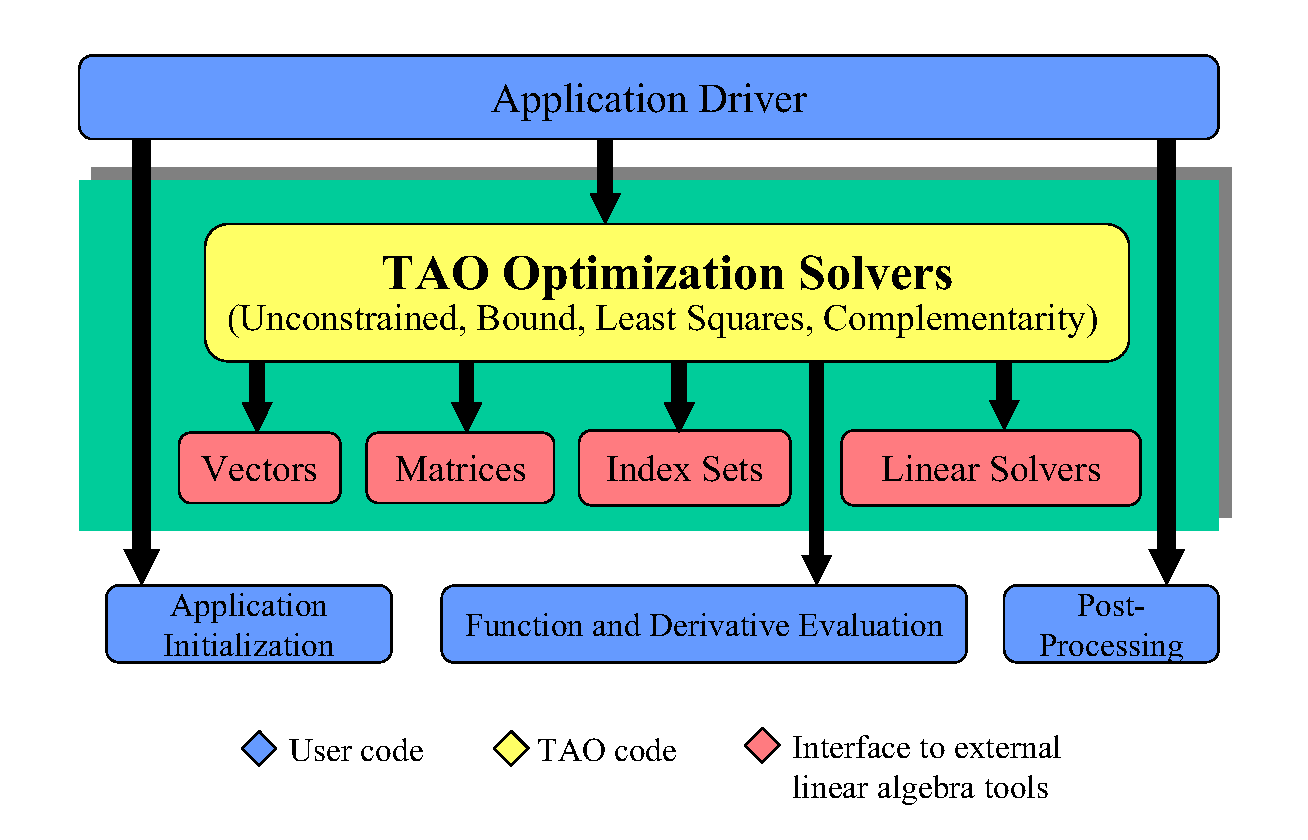
\includegraphics[height=3.5in,clip]{taofig.eps}}
%\caption{TAO Design}
%\label{tao:design}
%\end{figure}

\begin{figure}
\centerline{\epsfysize=3.5in \epsfbox{taofig.eps}}
\caption{TAO Design}
\label{tao:design}
\end{figure}


The TAO solvers use four fundamental objects to define and solve
optimization problems: vectors, index sets, matrices, and linear
solvers.  The concepts of vectors and matrices are standard, while an
index set refers to a set of integers used to identify particular
elements of vectors or matrices.  An optimization algorithm is a
sequence of well defined operations on these objects.  These
operations include vector sums, inner products, and matrix-vector
multiplication.  TAO makes no assumptions about the representation of
these objects by passing pointers to data-structure-neutral objects
for the execution of these numerical operations.

With sufficiently flexible abstract interfaces, TAO can support a
variety of implementations of data structures and algorithms.  These
abstractions allow us to more easily experiment with a range of
algorithmic and data structure options for realistic problems, such as
within this case study.  Such capabilities are critical for making
high-performance optimization software adaptable to the continual
evolution of parallel and distributed architectures and the research
community's discovery of new algorithms that exploit their features.

Our current TAO implementation uses the parallel system
infrastructure and linear algebra objects offered by PETSc,
which uses MPI \cite{using-mpi} for all interprocessor communication.
The PETSc package supports objects for vectors, matrices, index 
sets, and linear solvers.

The TAO design philosophy eliminates some of the barriers in using
independently developed software components by accepting data that is
independent of representation and calling sequence written for
particular data formats.  The user can initialize an application with
external frameworks, provide function information to a TAO solver, and
call TAO to solve the application problem.

The use of abstractions for matrices and vectors in TAO optimization
software also enables us to leverage automatic differentiation
technology to facilitate the parallel computation of gradients and
Hessians needed within optimization algorithms.  We have demonstrated
the viability of this approach through preliminary interfacing between
TAO solvers and the automatic differentiation tools ADIFOR and ADIC.
We are currently working on developing TAO interfaces that use special
problem features (for example, partial separability, stencil
information) in automatic differentiation computations.

\section{Performance Results}

A major concern in the TAO project is the performance and scalability
of optimization algorithms on large problems.  In this section we
focus on the GPCG (gradient projection, conjugate gradient) algorithm
for the solution of bound-constrained convex quadratic programming
problems.  Originally developed by Mor\'e and Toraldo
\cite{more-toraldo}, the GPCG algorithm was designed for large-scale
problems but had only been implemented for a single processor.  GPCG
combines the advantages of the identification properties of the
gradient projection method with the finite termination properties of
the conjugate gradient method.  Moreover, the performance of the
TAO implementation on large optimization problems is noteworthy.

%\begin{figure}[tb]
%\centering{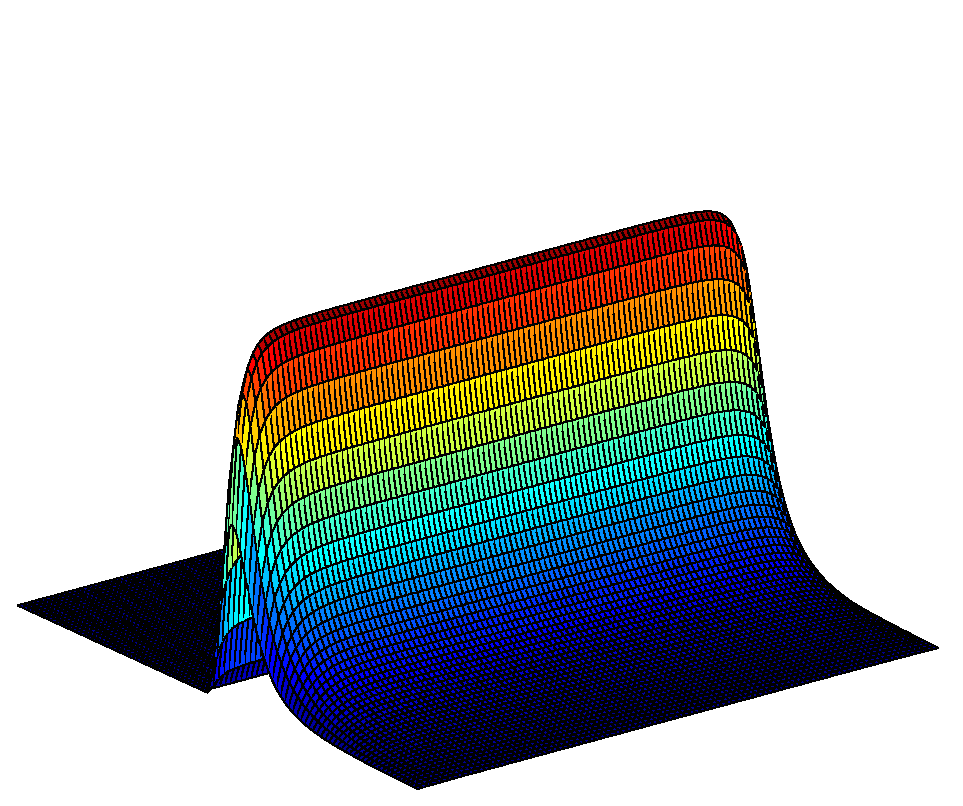
\includegraphics[height=3.0in]{pjb.eps}}
%\caption{The journal bearing problem with $\epsilon$ = 0.9}
%\label{dpjb}
%\end{figure}

\begin{figure}[tb]
\centerline{\epsfysize=3.0in \epsfbox{pjb.eps}}
\caption{The journal bearing problem with $\epsilon$ = 0.9}
\label{dpjb}
\end{figure}



We illustrate the performance of the GPCG algorithm by 
presenting results for a journal bearing problem
with over 2.5 million variables.
The journal bearing problem
is a finite element approximation to a variational problem 
over a rectangular two-dimensional grid.  A
grid with $1600$ points in each direction, for example, is formulated
as a bound constrained quadratic problem with $1600^2=2,560,000$
variables.
The triangulation of the grid results in a matrix that has the
usual five diagonal nonzero structure that arises
from a difference approximation to the Laplacian operator.
The journal bearing problem contains an eccentricity parameter,
$\varepsilon \in (0,1)$, that influences the number of active
variables at the solution and the difficulty in solving it.
Figure \ref{dpjb} shows the solution of the journal bearing problem
for $ \varepsilon = 0.9 $. The steep gradient in the solution
makes this problem a difficult benchmark.

The performance results in Table \ref{flops} are noteworthy is several
ways.  First of all, the number of faces visited by GPCG is remarkably
small.  Other strategies can lead to a large number of gradient
projection iterates, but the GPCG algorithm is remarkably efficient.
Another interesting aspect of these results is that due to the low
memory requirements of iterative solvers, we were able to solve these
problems with only $ p = 8 $ processors.  Strategies that rely on
direct solvers are likely to need significantly more storage, and thus
more processors.  Finally, these results show that the GPCG
implementation has excellent efficiency.  For example, the efficiency
of GPCG with respect to $ p = 8 $ processors ranges between $ 70\% $
and $ 100\% $ when $ \varepsilon = 0.1 $.  This sustained efficiency
is remarkable since the GPCG algorithm is solving a sequence of linear
problems with a coefficient matrix set to the submatrix of the Hessian
matrix with respect to the free variables for the current iterate.
Thus, our implementation's repartitioning of submatrices effectively
deals with the load-balancing problem that is inherent in the GPCG
algorithm.

\begin{table}[htb]
\begin{center}
\begin{tabular}{| c r | c c r c r |}
\hline
\multicolumn{1}{|c}{$ \varepsilon $} & 
\multicolumn{1}{c|}{$ p $} & 
\multicolumn{1}{c}{faces} &
\multicolumn{1}{c}{$n_{CG}$} & 
\multicolumn{1}{c}{time} &
\multicolumn{1}{c}{$t_{CG}$\%} & 
\multicolumn{1}{c|}{$ \cal E $} \\ \hline
0.1  & 8 & 46 & 431 & 7419 & 86 & 100  \\ 
0.1  & 16 & 45 & 423 & 3706 & 83 & 100  \\
0.1  & 32 & 45 & 427 & 2045 & 82 & 91 \\
0.1  & 64 & 45 & 427 & 1279 & 82 & 73 \\
\hline
0.9  & 8 & 37 & 105 & 2134 & 70 & 100 \\
0.9  & 16 & 37 & 103 & 1124 & 71 & 95 \\
0.9  & 32 & 38 & 100 & 618 & 69 & 86 \\
0.9  & 64 & 38 & 99 & 397 & 68 & 67 \\
\hline
\end{tabular}
\caption{Performance of GPCG on the journal bearing problem
with $ 2.56 \cdot 10^6 $ variables.}
\label{flops}
\end{center}
\end{table}




An important aspect of our results that is not
apparent from Table \ref{flops} is that 
for these results we were able to experiment easily 
with all the preconditioners offered by PETSc.
In particular, we were able to compare the diagonal Jacobi
preconditioner with block Jacobi and overlapping additive Schwarz
preconditioners that use a zero-fill ILU solver in each block.  We
also experimented with a parallel zero-fill incomplete Cholesky preconditioner
provided by a PETSc interface to the BlockSolve95~\cite{bs-user-ref}
package of Jones and
Plassmann.  Interestingly enough, the diagonal Jacobi preconditioner
achieved better performance on this problem.



%%% Local Variables: 
%%% mode: latex
%%% TeX-master: "manual_tex"
%%% End: 

\chapter{Getting Started}
\label{chapter:intro_tao}

TAO can be used on a personal
computer with a single processor or within a parallel environment.  
Its basic usage involves only a few commands, but fully 
understanding its usage requires time.
Application programmers can easily begin to use TAO by working with 
the examples provided and then gradually learn more details according to
their needs.  The current version of TAO and the most recent help 
concerning installation and usage can be found at  
\url{https://www.mcs.anl.gov/research/projects/tao/}.

See the PETSc users manual and \url{https://www.mcs.anl.gov/petsc} for how to install and start using PETSc/TAO.

\section{Writing Application Codes with TAO}

Examples throughout the library demonstrate the software usage and
can serve as templates for developing custom applications.  We suggest
that new TAO users examine programs in
\begin{verbatim}
   ${PETSC_DIR}/src/tao/<unconstrained,bound,..>/tutorials.
\end{verbatim} 
The HTML version of the manual pages located at
\begin{verbatim}
   ${PETSC_DIR}/docs/manpages/index.html
\end{verbatim} % To fool the coloring algorithm $
\noindent
and
\begin{verbatim}
   https://www.mcs.anl.gov/petsc/documentation/index.html
\end{verbatim}
\noindent
provides indices (organized by both routine names and concepts) to the
tutorial examples.

We suggest the following procedure for writing a new application
program using TAO:

\begin{enumerate}
\item Install PETSc/TAO according to the instructions in
  \url{https://www.mcs.anl.gov/petsc/documentation/installation.html}.
\item Copy an example and makefile from the directories
\begin{verbatim}
   ${PETSC_DIR}/src/tao/<unconstrained,bound,..>/tutorials.
\end{verbatim} 
  compile the example, and run the program. 
\item Select the example program matching the application most
  closely, and use it as a starting point for developing a customized
  code.
\end{enumerate}

\section{A Simple TAO Example}
\label{sec:simple}

To help the user start using TAO immediately, we introduce here a simple
uniprocessor example. Please read Section~\ref{chapter:tao_solver} for a 
more in-depth discussion on using the TAO solvers.
The code presented in Figure~\ref{fig:example1} minimizes the
extended Rosenbrock function $f: \Re^n \to \Re$ defined by
\[
 f(x) = 
 \sum_{i=0}^{m-1} \left( \alpha(x_{2i+1}-x_{2i}^2)^2 + (1-x_{2i})^2 \right),
\]
where $n = 2m$ is the number of variables.  Note that while we use the C 
language to introduce the TAO software, the package is fully usable from 
C++ and Fortran77/90.  Section~\ref{chapter:fortran} discusses additional 
issues concerning Fortran usage.

\afterpage{
\begin{figure}[H]
  {\footnotesize \verbatiminput{rosenbrock1.c}}
\caption{Example of Uniprocessor TAO Code\label{fig:example1}}
\end{figure}
}


The code in Figure~\ref{fig:example1} contains many of the components
needed to write most TAO programs and thus is illustrative of the
features present in complex optimization problems.  Note that for
display purposes we have omitted some nonessential lines of code as well as the
(essential) code required for the routine \texttt{FormFunctionGradient},
which evaluates the function and gradient, and the code for
\texttt{FormHessian}, which evaluates the Hessian matrix for Rosenbrock's
function. The complete code is available in \url{$TAO\_DIR/src/unconstrained/tutorials/rosenbrock1.c}. %$
The following sections annotates the lines of code in
Figure~\ref{fig:example1}.

\section{Include Files}

The include file for TAO should be used via the statement
\begin{verbatim}
   #include <petsctao.h>
\end{verbatim}
\noindent
The required lower-level include files are automatically included
within this high-level file.

\section{TAO Solvers}

Many TAO applications will follow an ordered set of procedures for 
solving an optimization problem:
The user creates a \texttt{Tao} context and selects a default algorithm. 
Call-back routines as well as vector (\texttt{Vec}) and matrix (\texttt{Mat}) 
data structures are then set.  These call-back routines will be used for 
evaluating the objective function, gradient, and perhaps the Hessian 
matrix.  The user then invokes TAO to solve the optimization problem and 
finally destroys
the \texttt{Tao} context. A list of the necessary functions for 
performing these steps
using TAO are shown in Figure \ref{fig:tao_commands}.  Details of these commands are presented in
Chapter~\ref{chapter:tao_solver}.

\findex{TaoCreate()} \findex{TaoSetObjectiveAndGradientRoutine()}
\findex{TaoSetRoutine()} \findex{TaoSolve()}
\findex{TaoDestroy()} \findex{TaoSetInitialVector()}
\begin{figure}[H]
\begin{verbatim}
   TaoCreate(MPI_Comm comm, Tao *tao); 
   TaoSetType(Tao tao, TaoType type);
   TaoSetInitialVector(Tao tao, Vec x);
   TaoSetObjectiveAndGradientRoutine(Tao tao, 
        PetscErrorCode (*FormFGradient)(Tao,Vec,PetscReal*,Vec,void*), 
        void *user);
   TaoSetHessianRoutine(Tao tao, Mat H, Mat Hpre,
        PetscErrorCode (*FormHessian)(Tao,Vec,Mat,Mat,
        void*), void *user);
   TaoSolve(Tao tao);
   TaoDestroy(Tao tao);
\end{verbatim}
\caption{Commands for Solving an Unconstrained Optimization Problem
\label{fig:tao_commands}}
\end{figure}

Note that the solver algorithm selected through the function 
\texttt{TaoSetType()} can be overridden
at runtime by using an options database.  Through this
database, the user not only can select a minimization method (e.g.,
limited-memory variable metric, conjugate gradient, Newton with line
search or trust region) but also can prescribe the convergence
tolerance, set various monitoring routines, set iterative methods
and preconditions for solving the linear systems, and so forth.  See 
Chapter~\ref{chapter:tao_solver} for more information on the 
solver methods available in TAO.

\section{Function Evaluations}

Users of TAO are required to provide routines that perform function
evaluations. Depending on the solver chosen, they may also have to
write routines that evaluate the gradient vector and Hessian matrix.

\section{Programming with PETSc}
\label{sec:tao_programming}
TAO relies heavily on PETSc not only for its vectors, matrices, and linear
solvers but also for its programming utilities such as command line option 
handling, error handling, and compiling system.  We provide here a quick 
overview of some of these PETSc features.  Please refer to the PETSc 
manual \cite{petsc-user-ref} for a more in-depth
discussion of PETSc.

\subsection*{Vectors}

In the example in Figure \ref{fig:example1}, the vector data structure
(\texttt{Vec}) is used to store the solution and gradient for the TAO
unconstrained minimization solvers.  A new parallel or sequential
vector \texttt{x} of global dimension \texttt{M} is created with the
command 
\begin{verbatim}
   info = VecCreate(MPI_Comm comm,int m,int M,Vec *x);
\end{verbatim}
\noindent
where \texttt{comm} denotes the MPI communicator. The type of storage
for the vector may be set with calls either to \texttt{VecSetType()}
or to \texttt{VecSetFromOptions()}.  Additional vectors of the same type
can be formed with 
\begin{verbatim}
   info = VecDuplicate(Vec old,Vec *new);
\end{verbatim}
\noindent
The commands
\begin{verbatim}
   info = VecSet(Vec X,PetscScalar value);
   info = VecSetValues(Vec x,int n,int *indices,
                       Scalar *values,INSERT_VALUES);
\end{verbatim}
\noindent
respectively set all the components of a vector to a particular scalar
value and assign a different value to each component.  More detailed
information about PETSc vectors, including their basic operations,
scattering/gathering, index sets, and distributed arrays, may be found
in the PETSc users manual \cite{petsc-user-ref}.

\subsection*{Matrices}

Usage of matrices and vectors is similar. \sindex{matrix} 
The user can create a new parallel or sequential matrix \texttt{H} with 
\texttt{M} global rows and \texttt{N} global columns, with the routines

\begin{verbatim}
   ierr = MatCreate(MPI_Comm comm,Mat *H);
   ierr = MatSetSizes(H,PETSC_DECIDE,PETSC_DECIDE,M,N);
\end{verbatim}
\noindent
where the matrix format can be specified at runtime.  The user could
alternatively specify each processes's number of local rows and columns
using \texttt{m} and \texttt{n} instead of \texttt{PETSC\_DECIDE}.  
\texttt{H} can then be used to store
the Hessian matrix, as indicated by the call to
\texttt{TaoSetHessianMat()}.  Matrix entries can be set with the
command
\begin{verbatim}
   ierr = MatSetValues(Mat H,PetscInt m,PetscInt *im, PetscInt n,
                       PetscInt *in, PetscScalar *values,INSERT_VALUES);
\end{verbatim}
\noindent
After %\findex{MatSetValues()} 
all elements have been inserted into the
matrix, it must be processed with the pair of commands

\begin{verbatim}
   ierr = MatAssemblyBegin(Mat H,MAT_FINAL_ASSEMBLY);
   ierr = MatAssemblyEnd(Mat H,MAT_FINAL_ASSEMBLY);
\end{verbatim}
\noindent
The PETSc users manual \cite{petsc-user-ref} discusses
various matrix formats as
well as the details of some basic matrix manipulation routines.


\subsection*{The Options Database}
\label{sec:options}
A TAO application can access the command line options presented at
runtime through the PETSc options database. This database gives the application
author the ability to set and change application parameters without
the need to recompile the application. For example, 
an application may have a grid discretization parameter \texttt{nx}
that can be set with the command line option \texttt{-nx <integer>}.
The application can read this option with the following line of code:
\begin{verbatim}
   PetscOptionsGetInt(NULL,NULL, "-nx", &nx, &flg);
\end{verbatim}
\noindent
If the command line option is present, the variable \texttt{nx} is set
accordingly; otherwise, \texttt{nx} remains unchanged. A complete
description of the options database may be found in the PETSc users
manual \cite{petsc-user-ref}.

\subsection*{Error Checking}

All TAO commands begin with the \texttt{Tao} prefix and return an
integer indicating whether an error has occurred during the call.  The
error code equals zero after the successful completion of the routine
and is set to a nonzero value if an error has been detected.  The
macro \texttt{CHKERRQ(ierr)} checks the value of \texttt{ierr} and calls an
error handler upon error detection.  \texttt{CHKERRQ()} should be used after
all subroutines to enable a complete error traceback.

In Figure \ref{fig:traceback} we indicate a traceback generated by
error detection within a sample program. The error occurred on line
2110 of the file \texttt{\$\{PETSC\_DIR\}/src/mat/inter\-face/mat\-rix.c} in the
routine \texttt{MatMult()} and was caused by failure to assemble the 
matrix in the Hessian evaluation routine.
The \texttt{MatMult()} routine was called from
the \texttt{TaoSolve\_NLS()} routine, which was in turn called on line 
154 of \texttt{TaoSolve()} from the \texttt{main()} routine 
in the program \texttt{rosenbrock1.c}.  The PETSc users
manual \cite{petsc-user-ref} provides further details
regarding error checking, including
information about error handling in Fortran.

\begin{figure}[htb]
{\footnotesize
\begin{verbatim}
> rosenbrock1 -tao_type nls
[0]PETSC ERROR: --------------------- Error Message ------------------------------------
[0]PETSC ERROR: Object is in wrong state!
[0]PETSC ERROR: Not for unassembled matrix!
[0]PETSC ERROR: ------------------------------------------------------------------------
[0]PETSC ERROR: Petsc Development HG revision: b95ffff514b66a703d96e6ae8e78ea266ad2ca19
[0]PETSC ERROR: See docs/changes/index.html for recent updates.
[0]PETSC ERROR: See docs/faq.html for hints about trouble shooting.
[0]PETSC ERROR: See docs/index.html for manual pages.
[0]PETSC ERROR: ------------------------------------------------------------------------
[0]PETSC ERROR: Libraries linked from petsc/arch-linux2-c-debug/lib
[0]PETSC ERROR: Configure run at Tue Jul 19 14:13:14 2011
[0]PETSC ERROR: Configure options --with-shared-libraries --with-dynamic-loading
[0]PETSC ERROR: ------------------------------------------------------------------------
[0]PETSC ERROR: MatMult() line 2110 in petsc/src/mat/interface/matrix.c
[0]PETSC ERROR: TaoSolve_NLS() line 291 in src/unconstrained/impls/nls/nls.c
[0]PETSC ERROR: TaoSolve() line 154 in src/interface/tao.c
[0]PETSC ERROR: main() line 94 in src/unconstrained/tutorials/rosenbrock1.c
application called MPI_Abort(MPI_COMM_WORLD, 73) - process 0
\end{verbatim}
}
\caption{Example of Error Traceback}
\label{fig:traceback}
\end{figure}

When running the debugging version of the TAO software (PETSc configured 
with the (default) \texttt{--with-debugging} option), checking is performed for 
memory corruption
(writing outside of array bounds, etc). The macros \texttt{CHKMEMQ} and
\texttt{CHKMEMA} can be called anywhere in the code and, when used together 
with the command line option \texttt{-malloc\_debug}, check the current
status of the memory for corruption.  By putting several (or many) of
these macros into an application code, one can usually track
down the code segment where corruption has occurred.

\subsection*{Parallel Programming}

Since TAO uses the message-passing model for parallel programming and
employs MPI for all interprocessor communication, the user is free to
employ MPI routines as needed throughout an application code.
By default, however, the user is shielded from many of the details of
message passing within TAO, since these are hidden within parallel
objects, such as vectors, matrices, and solvers.  In addition, TAO
users can interface to external tools, such as the generalized vector
scatters/gathers and distributed arrays within PETSc, for assistance in
managing parallel data.

%\sindex{collective operations} 
The user must specify a communicator
upon creation of any PETSc or TAO object (such as a vector, matrix, or 
solver)
to indicate the processors over which the object is to be distributed. 
For example, some commands for matrix, vector, and solver creation
are as follows.
\begin{verbatim}
   ierr = MatCreate(MPI_Comm comm,Mat *H);
   ierr = VecCreate(MPI_Comm comm,Vec *x);
   ierr = TaoCreate(MPI_Comm comm,Tao *tao); 
\end{verbatim}
\noindent
In most cases, the value for \texttt{comm} will be either 
\texttt{PETSC\_COMM\_SELF} for single-process objects or 
\texttt{PETSC\_COMM\_WORLD} for objects distributed over all processors.
The creation routines are collective over all processors in the
communicator; thus, all processors in the communicator {\em must} call
the creation routine.  In addition, if a sequence of collective
routines is being used, the routines {\em must} be called in the same
order on each processor.

%%% Local Variables: 
%%% mode: latex
%%% TeX-master: "manual_tex"
%%% End: 

%
% NOTES:  
%  - Be sure to place captions BEFORE labels in figures and tables!
%    Otherwise, numbering will be incorrect.  For example, use the following:
%       \caption{TAO Info}
%       \label{fig:taoinfo}
%  - Use \break to indicate a line break (needed to prevent long strings in
%    \tt mode from running of the page)
%
% ---------------------------------------------------------------

\chapter{Basic Usage of TAO Solvers}
%\sindex{continuous optimization}
\label{chapter:tao_solver}

TAO contains unconstrained minimization, bound constrained minimization, 
%nonlinear least squares, 
and nonlinear complementarity solvers.
The structure of these problems can differ significantly, 
but TAO has a similar interface to all of its solvers.  
Routines that most solvers have in common will be discussed in 
this chapter.
A complete list of options can be found by consulting the manual pages.
Many of the options can also be set at the command line.  These options
can also be found in manual pages or by
running a program with the {\tt -help} option.


\section{Initialize and Finalize}
The first TAO routine in any application should be {\tt TaoInitialize()}.
Most TAO programs begin with a call to
\findex{TaoInitialize()}
\begin{verbatim}
   info = TaoInitialize(int *argc,char ***argv,char *file_name, 
                        char *help_message);
\end{verbatim}
\noindent
This command initializes TAO, as well as MPI, PETSc, and other packages
to which TAO applications may link (if these have not yet
been initialized elsewhere).  
In particular, the arguments {\tt argc} and 
{\tt argv} are the command line arguments delivered in all C and C++
programs; these arguments initialize the options database.  
\sindex{command line arguments} The argument {\tt file\_name}
optionally indicates an alternative name for an options file, which by
default is called {\tt .petscrc} and resides in the user's home directory.

One of the last routines\findex{TaoFinalize()} that all TAO programs should 
call is 
\begin{verbatim}
   info = TaoFinalize();
\end{verbatim}
\noindent
This routine finalizes TAO and any other libraries that may have been
initialized during the {\tt TaoInitialize()} phase.
For example, {\tt TaoFinalize()}
calls {\tt MPI\_Finalize()} %\findex{MPI_Finalize()}
if {\tt TaoInitialize()}
began MPI. If MPI was initiated externally from TAO (by either
the user or another software package), then the user is
responsible for calling {\tt MPI\_Finalize()}. 

\section{Creation and Destruction}

A TAO solver can be created with
the command 
\findex{TaoCreate()}
\begin{verbatim}
   info = TaoCreate(MPI_Comm comm,TaoMethod method,TAO_SOLVER *newsolver);
\end{verbatim}
\noindent
The first argument in this routine is an MPI communicator indicating which
processes are involved in the solution process.  In
most cases, this should be set to {\tt MPI\_COMM\_WORLD}.
The second argument in this creation routine 
specifies the default method that should be be used to
solve the optimization problem.  
The third argument in {\tt TaoCreate()} is a pointer to a TAO solver
object.  This routine creates the object and returns it to the user.
The TAO object is then to be used in all TAO routines.

The various types of TAO solvers and the flags that identify them 
will be discussed in the following chapters.
The solution method should be carefully chosen depending upon
the problem that is being solved.  Some solvers, for instance, are meant for
problems with no constraints, while other solvers acknowledge constraints
in the problem and solve them accordingly.
The user must also be aware of the derivative information that is available.
Some solvers require second-order information, while other solvers require
only gradient or function information.
The {\tt TaoMethod} can also be set to {\tt TAO\_NULL} in the 
{\tt TaoCreate()} routine if the user selects a method at runtime using
the options database.
The command line option \texttt{-tao\_method} followed by an TAO method
will override any method specified by the second argument.
The command line option {\tt -tao\_method tao\_lmvm}, for instance,
will specify the limited memory variable metric method for unconstrained
optimization.  Note that the {\tt TaoMethod} variable is a string that requires
quotation marks in an application program, but quotation marks are not required
at the command line.
The method that TAO uses to solve an optimization problem can be changed at a later point
in the program with the command
\findex{TaoSetMethod()} {\tt TaoSetMethod()}, whose
arguments are a TAO solver
and a string that uniquely identifies a method for solving the problem.

Each TAO solver that has been created should also be destroyed using
the command 
\findex{TaoDestroy()}
\begin{verbatim}
   info = TaoDestroy(TAO_SOLVER solver);
\end{verbatim}
\noindent 
This routine frees the internal data structures used by the solver.


\section{Convergence}\label{sec:customize}

Although TAO and its solvers set default parameters 
that are useful
for many problems, it may be necessary for the user to modify these
parameters to change the behavior and convergence of various algorithms.

One convergence criterion for most algorithms concerns the
of digits of accuracy needed in the solution.  In particular,
one convergence test employed by TAO attempts to stop when
the error in the constraints is less than $\epsilon_{crtol}$,
 and either
\[\frac{ |f(X) - f(X^*)|}{ |f(X)| + 1} \leq \epsilon_{frtol}
\;\textnormal{or}\;
f(X) - f(X^*)  \leq \epsilon_{fatol}, \]
where $X^*$ is the current approximation to $X$.
TAO estimates $f(X) - f(X^*)$ with either 
the square of the norm of the gradient or the duality gap.
A relative tolerance of $\epsilon_{frtol}=0.01$ indicates that two
significant digits are desired in the objective function.
Each solver sets its own  convergence tolerances, but they can
be changed using the routine
{\tt TaoSetTolerances()}\findex{TaoSetTolerances()} \sindex{convergence tests}. 
Another set of convergence tolerances can be set with 
{\tt TaoSetGradientTolerances()}.\findex{TaoSetGradientTolerances()}
These tolerances terminate the solver when the norm of the gradient function
(or Lagrangian function for bound-constrained problems)
is sufficiently close to zero.

Other stopping criteria include a minimum trust region radius or 
a maximum number of iterations.  These parameters can be set with
the routines {\tt TaoSetTrustRegionTolerance()}\sindex{trust region}\findex{TaoSetTrustRegionTolerance}
and {\tt TaoSetMaximumIterates()}\findex{TaoSetMaximumIterates()}.
Similarly, a maximum number of function evaluations can be set 
with the command 
{\tt TaoSetMaximumFunctionEvaluations()}
\findex{TaoSetMaximumFunctionEvaluations()}.

\section{Viewing Solutions}

The routine
\begin{verbatim}
   int TaoSolveApplication(TAO_APPLICATION, TAO_SOLVER);
\end{verbatim}
\noindent
will apply the solver to the application that has been created by the user.

To see parameters and performance statistics for the solver, the
routine
\begin{verbatim}
   int TaoView(TAO_SOLVER);
\end{verbatim}
can be used.  This routine will display to standard output the number
of function evaluations need by the solver and other information
specific to the solver.

The progress of the optimization solver can be monitored with
the runtime option {\tt -tao\_monitor}.  Although monitoring routines
can be customized, the default monitoring routine will print out 
several relevant statistics to the screen.

The user also has access to information about the current solution.
The current iteration number, objective function value, gradient
norm, infeasibility norm, and step length 
can be retrieved with the command 
\findex{TaoGetSolutionStatus()}
\begin{verbatim}
   int TaoGetSolutionStatus(TAO_SOLVER tao, int* iterate, double* f, 
                            double* gnorm, double *cnorm, double *xdiff, 
                            TaoTerminateReason *reason)
\end{verbatim}
\noindent
The last argument returns
a code that indicates the reason that the solver terminated.  Positive 
numbers indicate that a solution has been found, while negative numbers
indicate a failure.  A list of reasons can be found in the manual page
for {\tt TaoGetTerminationReason()}.

The user set
vectors containing the solution and gradient before solving
the problem, but pointers to these vectors can also be retrieved with the
commands {\tt TaoGetSolution()}\findex{TaoGetSolution()}
and {\tt TaoGetGradient()}\findex{TaoGetGradient()}.  
Dual variables and other relevant information are also available. 
This information can be obtained during
user-defined routines such as a function evaluation and customized
monitoring routine, or after the solver has terminated.

%%% Local Variables: 
%%% mode: latex
%%% TeX-master: "manual_tex"
%%% End: 


\chapter{TAO Solvers}

\section{Unconstrained Minimization}
\label{chapter:unconstrained}
Unconstrained minimization is used to minimize a function of many variables
without any constraints on the variables, such as bounds.  The methods 
available in TAO for solving these problems can be classified according
to the amount of derivative information required:
\begin{enumerate}
\item Function evaluation only -- Nelder-Mead method ({\tt tao\_nm})
\item Function and gradient evaluations -- limited-memory, variable-metric 
method ({\tt tao\_lmvm}) and nonlinear conjugate gradient method 
({\tt tao\_cg})
\item Function, gradient, and Hessian evaluations -- Newton line-search 
method ({\tt tao\_nls}) and Newton trust-region method ({\tt tao\_ntr})
\end{enumerate}
The best method to use depends on the particular problem being solved
and the accuracy required in the solution.  If a Hessian evaluation 
routine is available, then the Newton line-search and Newton trust-region 
methods will be the best performers.  When a Hessian evaluation routine
is not available, then the limited-memory, variable-metric method is 
likely to perform best.  The Nelder-Mead method should be used only
as a last resort when no gradient information is available.

Each solver has a set of options associated with it that can be set with 
command line arguments.  A brief description of these algorithms and the 
associated options are discussed in this chapter.

\subsection{Nelder-Mead}
The Nelder-Mead algorithm \cite{nelder.mead:simplex} is a direct search method for finding a local
minimum of a function $f(x)$.  This algorithm does not require any gradient or Hessian 
information of $f$, and therefore has some expected advantages and disadvantages compared
to the other TAO solvers.  The obvious advantage is that it is easier to write an 
application when no derivatives need to be calculated.  The downside is that this algorithm can
be very slow to converge or can even stagnate, and performs poorly for large numbers of variables.

This solver keeps a set of $N+1$ sorted vectors ${x_1,x_2,\ldots,x_{N+1}}$ and their corresponding 
objective function values $f_1 \leq f_2 \leq \ldots \leq f_{N+1}$.  At each iteration, $x_{N+1}$ is removed from
the set and replaced with 
\[
x(\mu) = (1+\mu) \frac{1}{N} \sum_{i=1}^N x_i - \mu x_{N+1},
\]  
 
where $\mu$ can be one of ${\mu_0,2\mu_0,\frac{1}{2}\mu_0,-\frac{1}{2}\mu_0}$ depending upon the values of 
each possible $f(x(\mu))$.

The algorithm terminates when the residual  $f_{N+1} - f_1$ becomes sufficiently small.  Because of 
the way new vectors can be added to the sorted set, 
the minimum function value and/or the residual may not be impacted at each iteration.

There are two options that can be set specifically for the Nelder-Mead algorithm,
{\tt -tao\_nm\_lamda <value>} sets the initial set of vectors ($x_0$ plus 
{\tt value} in each cartesion direction), the default value is $1$.  
{\tt tao\_nm\_mu <value>} sets the value of $\mu_0$, 
the default is $\mu_0=1$.


\subsection{Limited-Memory, Variable-Metric Method}\sindex{line search}\sindex{gradients}

The limited-memory, variable-metric method solves the system of equations
\[
H_k d_k = -\nabla f(x_k),
\]
where $H_k$ is a positive definite approximation to the Hessian matrix 
obtained by using the BFGS update formula with a limited number of 
previous iterates and gradient evaluations.  The inverse of $H_k$ can 
readily be applied to obtain the direction $d_k$.  Having obtained the 
direction, a Mor\'{e}-Thuente line search is applied to compute a step
length, $\tau_k$, that approximately solves the one-dimensional 
optimization problem
\[
\min_\tau f(x_k + \tau d_k).
\]
The current iterate and Hessian approximation are updated and the process
is repeated until the method converges.  This algorithm is the default 
unconstrained minimization solver and can be selected using the 
TaoMethod {\tt tao\_lmvm}.  For best efficiency, function and gradient 
evaluations should be performed simultaneously when using this algorithm.

The primary factors determining the behavior of this algorithm are the 
number of vectors stored for the Hessian approximation and the scaling matrix
used when computing the direction.  The number of vectors stored can be set
with the command line argument {\tt -tao\_lmm\_vectors <int>}; $5$ is the 
default 
value.  Increasing the number of vectors results in a better Hessian 
approximation and can decrease the number of iterations required to compute
a solution to the optimization problem.  However, as the number of vectors
increases, more memory is consumed and each direction calculation takes
longer to compute.  Therefore, a trade off must be made between the 
quality of the Hessian approximation, the memory requirements, and
the time to compute the direction.

During the computation of the direction, the inverse of an initial 
Hessian approximation $H_{0,k}$ is applied.  The choice of $H_{0,k}$
has a significant impact on the quality of the direction obtained
and can result in a decrease in the number of function and gradient 
evaluations required to solve the optimization problem.  However,
the calculation of $H_{0,k}$ at each iteration can have a significant 
impact on the time required to update the limited-memory BFGS 
approximation and the cost of obtaining the direction.  By default, 
$H_{0,k}$ is a diagonal matrix obtained from the diagonal entries
of a Broyden approximation to the Hessian matrix.  The calculation
of $H_{0,k}$ can be modified with the command line argument 
{\tt -tao\_lmm\_scale\_type <none,scalar,broyden>}.  Each scaling 
method is described below.  The {\tt scalar} and {\tt broyden} 
techniques are inspired by \cite{Gilbert-Lemarechal}.

\begin{description}
\item[{\tt none}]  This scaling method uses the identity matrix as 
$H_{0,k}$.  No extra computations are required when obtaining the 
search direction or updating the Hessian approximation.  However, 
the number of functions and gradient evaluations required to converge
to a solution is typically much larger than the number required when 
using other scaling methods.
\item[{\tt scalar}]  This scaling method uses a multiple of the identity 
matrix as $H_{0,k}$.  The scalar value $\sigma$ is chosen by solving the 
one-dimensional optimization problem
\[
\min_\sigma \|\sigma^\alpha Y - \sigma^{\alpha - 1} S\|_F^2,
\]
where $\alpha \in [0,1]$ is given, and $S$ and $Y$ are the matrices of 
past iterate and gradient information required by the limited-memory
BFGS update formula.  The optimal value for $\sigma$ can be written
down explicitly.  This choice of $\sigma$ attempts to satisfy the 
secant equation $\sigma Y = S$.  Since this equation cannot typically
be satisfied by a scalar, a least norm solution is computed.  The amount 
of past iterate and gradient information used is set by the command line 
argument {\tt tao\_lmm\_scalar\_history <int>}, which must be less than 
or equal to the number of vectors kept for the BFGS approximation.  
The default value is 5.  The choice for $\alpha$ is made with the command 
line argument {\tt tao\_lmm\_scalar\_alpha <double>}; $1$ is the default
value.  This scaling method offers a good compromise between no scaling 
and {\tt broyden} scaling.
\item[{\tt broyden}] This scaling method uses a positive-definite diagonal 
matrix obtained from the diagonal entries of the Broyden approximation to 
the Hessian for the scaling matrix.  The Broyden approximation is a 
family of approximations parametrized by a constant $\phi$; $\phi = 0$ 
gives the BFGS formula and $\phi = 1$ gives the DFP formula.  The value 
of $\phi$ is set with the command line argument 
{\tt -tao\_lmm\_broyden\_phi <double>}.  The default value for $\phi$ 
is $0.125$.  This scaling method requires the most computational effort 
of available choices, but typically results in a significant reduction 
in the number of function and gradient evaluations taken to compute a 
solution.
\end{description}

An additional rescaling of the diagonal matrix can be applied to further
improve performance when using the {\tt broyden} scaling method.  The
rescaling method can be set with the command line argument 
{\tt -tao\_lmm\_rescale\_type <none,scalar,gl>}; {\tt scalar} is the 
default rescaling method.  The rescaling method applied can have a large 
impact on the number of function and gradient evaluations necessary to 
compute a solution to the optimization problem, but increases the time
required to update the BFGS approximation.  Each rescaling method is 
described below.  These techniques are inspired by \cite{Gilbert-Lemarechal}.

\begin{description}
\item[{\tt none}] This rescaling method does not modify the diagonal scaling
matrix.
\item[{\tt scalar}] This rescaling method chooses a scalar value $\sigma$ by 
solving the one-dimensional optimization problem
\[
\min_\sigma \|\sigma^\alpha H_{0,k}^{\beta} Y - \sigma^{\alpha - 1} H_{0,k}^{\beta - 1} S\|_F^2,
\]
where $\alpha \in [0,1]$ and $\beta \in [0,1]$ are given, $H_{0,k}$ is the 
positive-definite diagonal scaling matrix computed by using the Broyden 
update, and $S$ and $Y$ are the matrices of past iterate and gradient
information required by the limited-memory BFGS update formula.  This 
choice of $\sigma$ attempts to satisfy the secant equation 
$\sigma H_{0,k} Y = S$.  Since this equation cannot typically be satisfied 
by a scalar, a least norm solution is computed.  The scaling matrix used is 
then $\sigma H_{0,k}$.  The amount of past iterate and gradient information 
used is set by the command line argument 
{\tt tao\_lmm\_rescale\_history <int>}, which must be less than or equal
to the number of vectors kept for the BFGS approximation.  The default value 
is 5.  The choice for $\alpha$ is made with the command
line argument {\tt tao\_lmm\_rescale\_alpha <double>}; $1$ is the default
value.  The choice for $\beta$ is made with the command line argument 
{\tt tao\_lmm\_rescale\_beta <double>}; $0.5$ is the default value.
\item[{\tt gl}] This scaling method is the same as the {\tt scalar} rescaling 
method, but the previous value for the scaling matrix $H_{0,k-1}$ is used when 
computing $\sigma$.  This is the rescaling method suggested in 
\cite{Gilbert-Lemarechal}.
\end{description}

Finally, a limit can be placed on the difference between the scaling
matrix computed at this iteration and the previous value for the
scaling matrix.  The limiting type can be set with the command line 
argument {\tt -tao\_lmm\_limit\_type <none,average,relative,absolute>};
{\tt none} is the default value.  Each of these methods is described 
below when using the {\tt scalar} scaling method.  The techniques are
the same when using the {\tt broyden} scaling method, but are applied
to each entry in the diagonal matrix.

\begin{description}
\item[{\tt none}] Set $\sigma_k = \sigma$, where $\sigma$ is the value
computed by the scaling method.
\item[{\tt average}] Set $\sigma_k = \mu \sigma + (1 - \mu) \sigma_{k-1}$, 
where $\sigma$ is the value computed by the scaling method, $\sigma_{k-1}$ is
the previous value, and $\mu \in [0,1]$ is given.
\item[{\tt relative}] Set $\sigma_k = \mbox{median}\left\{ (1 - \mu) \sigma_{k-1}, \sigma, (1+\mu) \sigma_{k-1}\right\}$, 
where $\sigma$ is the value computed by the scaling method, $\sigma_{k-1}$ is 
the previous value, and $\mu \in [0,1]$ is given.
\item[{\tt absolute}] Set $\sigma_k = \mbox{median}\left\{\sigma_{k-1} - \nu, \sigma, \sigma_{k-1} + \nu\right\}$, 
where $\sigma$ is the value computed by the scaling method, $\sigma_{k-1}$ is 
the previous value, and $\nu$ is given.
\end{description}
The value for $\mu$ is set with the command line argument 
{\tt -tao\_lmm\_limit\_mu <double>}; $1$ is the default value.
The value for $\nu$ is set with the command line argument 
{\tt -tao\_lmm\_limit\_nu <double>}.  The default value is 100.  

The default values for the scaling are based on many tests using the
unconstrained problems from the MINPACK-2 test set.  These tests were
used to narrow the choices to a few sets of values.  These values were
then run on the unconstrained problems from the CUTEr test set to
obtain the default values supplied.

\begin{table}[h]
\caption{Summary of {\tt lmvm} options}
\begin{tabular}{l|p{1.5in}|l|p{2.0in}}
Name & Value & Default & Description \\
{\tt -tao\_lmm\_vectors} & int & 5 & Number of vectors for Hessian approximation \\
{\tt -tao\_lmm\_scale\_type} & none, scalar, broyden & broyden & Type of scaling method to use \\
{\tt -tao\_lmm\_scalar\_history} & int & 5 & Number of vectors to use when scaling \\
{\tt -tao\_lmm\_scalar\_alpha} & double & 1 & Value of $\alpha$ for scalar scaling method \\
{\tt -tao\_lmm\_broyden\_phi} & double & 0.125 & Value of $\alpha$ for scalar scaling method \\
{\tt -tao\_lmm\_rescale\_type} & none, scalar, gl & scalar & Type of rescaling method to use \\
{\tt -tao\_lmm\_rescale\_history} & int & 5 & Number of vectors to use when rescaling \\
{\tt -tao\_lmm\_rescale\_alpha} & double & 1 & Value of $\alpha$ for rescaling method \\
{\tt -tao\_lmm\_rescale\_beta} & double & 0.5 & Value of $\beta$ for rescaling method \\
{\tt -tao\_lmm\_limit\_type} & none, average, relative, absolute & none & Type of limit to impose on scaling matrix \\
{\tt -tao\_lmm\_limit\_mu} & double & 1 & Value of $\mu$ for limit type\\
{\tt -tao\_lmm\_limit\_nu} & double & 100 & Value of $\nu$ for limit type\\
\end{tabular}
\end{table}

\subsection{Nonlinear Conjugate Gradient Method}\sindex{line search}\sindex{gradients}

The nonlinear conjugate gradient method can be viewed as an extensions of the 
conjugate gradient method for solving symmetric, positive-definite linear 
systems of equations.  This algorithm requires only function and gradient 
evaluations as well as a line search.  The TAO implementation uses a 
Mor\'{e}-Thuente line search to obtain the step length.  The nonlinear 
conjugate gradient method can be selected by using the TaoMethod 
{\tt tao\_cg}.  For the best efficiency, function and gradient evaluations 
should be performed simultaneously when using this algorithm.

Five variations are currently supported by the TAO implementation: the 
Fletcher-Reeves method, the Polak-Ribi\'ere method, the Polak-Ribi\'ere-Plus 
method\cite{NW99}, the Hestenes-Stiefel method, and the Dai-Yuan method.  
These conjugate gradient methods can be specified by using the command line 
argument {\tt tao\_cg\_type <fr,pr,prp,hs,dy>}, respectively.  The default 
value is {\tt prp}.  

The conjugate gradient method incorporates automatic restarts when successive 
gradients are not sufficiently orthogonal.  TAO measures the orthogonality by 
dividing the inner product of the gradient at the current point and the 
gradient at the previous point by the square of the Euclidean norm of 
the gradient at the current point.  When the absolute value of this 
ratio is greater than $\eta$, the algorithm restarts using the gradient 
direction.  The parameter $\eta$ can be set using the command line argument 
{\tt -tao\_cg\_eta <double>}; 0.1 is the default value.  

\subsection{Newton Line-Search Method}\sindex{Newton method}\sindex{line search}

The Newton line-search method solves the symmetric system of equations
\[
H_k d_k = -g_k
\]
to obtain a step $d_k$, where $H_k$ is the Hessian of the objective function
at $x_k$ and $g_k$ is the gradient of the objective function at $x_k$.
For problems where the Hessian matrix is indefinite, the perturbed system
of equations
\[
(H_k + \rho_k I) d_k = -g_k
\]
is solved to obtain the direction, where $\rho_k$ is a positive constant.
If the direction computed is not a descent direction, the (scaled) steepest 
descent direction is used instead.  Having obtained the direction, 
a Mor\'{e}-Thuente line search is applied to obtain a step length, 
$\tau_k$, that approximately solves the one-dimensional optimization 
problem
\[
\min_\tau f(x_k + \tau d_k).
\]
The Newton line-search method can be set using the TaoMethod {\tt tao\_nls}.
For the best efficiency, function and gradient evaluations should be 
performed simultaneously when using this algorithm.

The system of equations is approximately solved by applying the conjugate 
gradient method, Steihaug-Toint conjugate gradient method, generalized 
Lanczos method, or an alternative Krylov subspace method 
supplied by PETSc.  The method used to solve the systems of equations is 
specified with the command line argument 
{\tt -tao\_nls\_ksp\_type <cg,stcg,gltr,petsc>}; {\tt cg} 
is the default.  When the type is set to {\tt petsc}, the method set with 
the PETSc {\tt -ksp\_type} command line argument is used.  For example, to 
use GMRES as the linear system solver, one would use the the command line 
arguments {\tt -tao\_nls\_ksp\_type petsc -ksp\_type gmres}.  Internally,
the PETSc implementations for the conjugate gradient methods and the 
generalized Lanczos method are used.  See the PETSc manual for further 
information on changing the behavior of the linear system solvers.  

A good preconditioner reduces the number of iterations required to
solve the linear system of equations.  For the conjugate gradient
methods and generalized Lanczos method, this preconditioner must be
symmetric and positive definite.  The available options are to use no
preconditioner, the absolute value of the diagonal of the Hessian
matrix, a limited-memory BFGS approximation to the Hessian matrix, or
one of the other preconditioners provided by the PETSc package.  These
preconditioners are specified by the command line argument 
{\tt -tao\_nls\_pc\_type <none,ahess,bfgs,petsc>}, respectively. The
default is the {\tt bfgs} preconditioner.  When the preconditioner
type is set to {\tt petsc}, the preconditioner set with the PETSc 
{\tt -pc\_type} command line argument is used.  For example, to use an
incomplete Cholesky factorization for the preconditioner, one would
use the command line arguments 
{\tt -tao\_nls\_pc\_type petsc -pc\_type icc}.  See the PETSc manual 
for further information on changing the behavior of the preconditioners.

The choice of scaling matrix can have a significant impact on the quality 
of the Hessian approximation when using the {\tt bfgs} preconditioner and
affect the number of iterations required by the linear system solver.
The choices for scaling matrices are the same as those discussed for 
the limited-memory, variable-metric algorithm.  For Newton methods,
however, the option exists to use a scaling matrix based on the true
Hessian matrix.  In particular, the implementation supports using the 
absolute value of the diagonal of the Hessian matrix or the absolute 
value of the diagonal of the perturbed Hessian matrix.  The scaling 
matrix to use with the {\tt bfgs} preconditioner is set with the 
command line argument {\tt -tao\_nls\_bfgs\_scale\_type <bfgs,ahess,phess>}; 
{\tt phess} is the default.  The {\tt bfgs} scaling matrix is derived from 
the BFGS options.  The {\tt ahess} scaling matrix is the absolute value of 
the diagonal of the Hessian matrix.  The {\tt phess} scaling matrix is
the absolute value of the diagonal of the perturbed Hessian matrix.

The perturbation $\rho_k$ is added when the direction returned by the
Krylov subspace method is either not a descent direction, the Krylov method
diverged due to an indefinite preconditioner or matrix, or a direction of 
negative curvature was found.  In the two latter cases, if the step returned
is a descent direction, it is used during the line search.  Otherwise, a
steepest descent direction is used during the line search.  The perturbation
is decreased as long as the Krylov subspace method reports success and 
increased if further problems are encountered.  There are three cases:
initializing, increasing, and decreasing the perturbation.  These cases
are described below.
\begin{enumerate}
\item If $\rho_k$ is zero and a problem was detected with either the
direction on the Krylov subspace method, the perturbation is initialized to
\[
\rho_{k+1} = \mbox{median}\left\{\mbox{imin}, \mbox{imfac} * \|g(x_k)\|, \mbox{imax}\right\},
\]
where {\tt imin} is set with the command line argument 
{\tt -tao\_nls\_imin <double>} with a default value of $10^{-4}$,
{\tt imfac} by {\tt -tao\_nls\_imfac} with a default value of 0.1, and 
{\tt imax} by {\tt -tao\_nls\_imax} with a default value of 100.  
When using the {\tt gltr} method to solve the system of equations, an
estimate of the minimum eigenvalue $\lambda_1$ of the Hessian matrix 
is available.  This value is use to initialize the perturbation to
$\rho_{k+1} = \max\left\{\rho_{k+1}, -\lambda_1\right\}$.
\item If $\rho_k$ is nonzero and a problem was detected with either the 
direction or Krylov subspace method, the perturbation is increased to 
\[
\rho_{k+1} = \min\left\{\mbox{pmax}, \max\left\{\mbox{pgfac} * \rho_k, \mbox{pmgfac} * \|g(x_k)\|\right\}\right\},
\]
where {\tt pgfac} is set with the command line argument {\tt -tao\_nls\_pgfac}
with a default value of 10, {\tt pmgfac} by {\tt -tao\_nls\_pmgfac} with a
default value of 0.1, and {\tt pmax} by {\tt -tao\_nls\_pmax} with a default
value of 100.
\item If $\rho_k$ is nonzero and no problems were detected with either
the direction or Krylov subspace method, the perturbation is decreased to
\[
\rho_{k+1} = \min\left\{\mbox{psfac} * \rho_k, \mbox{pmsfac} * \|g(x_k)\|\right\},
\]
where {\tt psfac} is set with the command line argument {\tt -tao\_nls\_psfac}
with a default value of 0.4, and {\tt pmsfac} by {\tt -tao\_nls\_pmsfac} with
a default value of 0.1.  Moreover, if $\rho_{k+1} < \mbox{pmin}$ then 
$\rho_{k+1} = 0$, where {\tt pmin} is set with the command line argument 
{\tt -tao\_nls\_pmin} and has a default value of $10^{-12}$.
\end{enumerate}

When using {\tt stcg} or {\tt gltr} to solve the linear systems of equation,
a trust-region radius need to be initialized and updated.  This trust-region
radius limits the size of the step computed.  The method for initializing
the trust-region radius is set with the command line argument 
{\tt -tao\_nls\_init\_type <constant,direction,interpolation>};
{\tt interpolation}, which chooses an initial value based on the 
interpolation scheme found in \cite{CGT}, is the default.  This
scheme performs a number of function and gradient evaluations to determine 
a radius such that the reduction predicted by the quadratic model along the 
gradient direction coincides with the actual reduction in the nonlinear 
function.  The iterate obtaining the best objective function value is 
used as the starting point for the main line-search algorithm.  The 
{\tt constant} method initializes the trust-region radius by using 
the value specified with the {\tt -tao\_trust0 <double>} command line 
argument, where the default value is 100.  The {\tt direction} technique 
solves the first quadratic optimization problem by using a standard 
conjugate gradient method and initializes the trust-region to 
$\|s_0\|$.

Finally, the method for updating the trust-region radius is set with the 
command line argument 
{\tt -tao\_nls\_update\_type <step,reduction,interpolation>}; {\tt step} 
is the default.  The {\tt step} method updates the trust-region 
radius based on the value of $\tau_k$.  In particular,
\[
\Delta_{k+1} = \left\{\begin{array}{ll}
\omega_1 \mbox{min}(\Delta_k, \|d_k\|) & \mbox{if } \tau_k \in [0, \nu_1) \\
\omega_2 \mbox{min}(\Delta_k, \|d_k\|) & \mbox{if } \tau_k \in [\nu_1, \nu_2) \\
\omega_3 \Delta_k & \mbox{if } \tau_k \in [\nu_2, \nu_3) \\
\mbox{max}(\Delta_k, \omega_4 \|d_k\|) & \mbox{if } \tau_k \in [\nu_3, \nu_4) \\
\mbox{max}(\Delta_k, \omega_5 \|d_k\|) & \mbox{if } \tau_k \in [\nu_4, \infty)
\end{array}
\right.
\]
where $0 < \omega_1 < \omega_2 < \omega_3 = 1 < \omega_4 < \omega_5$ and
$0 < \nu_1 < \nu_2 < \nu_3 < \nu_4$ are constants.  The {\tt reduction} 
method computes the ratio of the actual reduction in the objective function 
to the reduction predicted by the quadratic model for the full step, 
$\kappa_k = \frac{f(x_k) - f(x_k + d_k)}{q(x_k) - q(x_k + d_k)}$, where 
$q_k$ is the quadratic model.  The radius is then updated as:
\[
\Delta_{k+1} = \left\{\begin{array}{ll}
\alpha_1 \mbox{min}(\Delta_k, \|d_k\|) & \mbox{if } \kappa_k \in (-\infty, \eta_1) \\
\alpha_2 \mbox{min}(\Delta_k, \|d_k\|) & \mbox{if } \kappa_k \in [\eta_1, \eta_2) \\
\alpha_3 \Delta_k & \mbox{if } \kappa_k \in [\eta_2, \eta_3) \\
\mbox{max}(\Delta_k, \alpha_4 \|d_k\|) & \mbox{if } \kappa_k \in [\eta_3, \eta_4) \\
\mbox{max}(\Delta_k, \alpha_5 \|d_k\|) & \mbox{if } \kappa_k \in [\eta_4, \infty)
\end{array}
\right.
\]
where $0 < \alpha_1 < \alpha_2 < \alpha_3 = 1 < \alpha_4 < \alpha_5$ and
$0 < \eta_1 < \eta_2 < \eta_3 < \eta_4$ are constants.  The {\tt interpolation}
method uses the same interpolation mechanism as in the initialization to
compute a new value for the trust-region radius.

\begin{table}[h]
\caption{Summary of {\tt nls} options}
\begin{tabular}{l|p{1.5in}|l|p{2.0in}}
Name & Value & Default & Description \\
{\tt -tao\_nls\_ksp\_type} & cg, stcg, gltr, petsc & cg & Type of Krylov subspace method to use when solving linear system \\
{\tt -tao\_nls\_pc\_type} & none, ahess, bfgs, petsc & bfgs & Type of preconditioner to use when solving linear system \\
{\tt -tao\_nls\_bfgs\_scale\_type} & ahess, phess, bfgs & phess & Type of scaling matrix to use with BFGS preconditioner \\
{\tt -tao\_nls\_sval} & double & $0$ & Initial perturbation value \\
{\tt -tao\_nls\_imin} & double & $10^{-4}$ & Minimum initial perturbation value \\
{\tt -tao\_nls\_imax} & double & $100$ & Maximum initial perturbation value \\
{\tt -tao\_nls\_imfac} & double & $0.1$ & Factor applied to norm of gradient when initializing perturbation \\
{\tt -tao\_nls\_pmax} & double & $100$ & Maximum perturbation when increasing value \\
{\tt -tao\_nls\_pgfac} & double & $10$ & Growth factor applied to perturbation when increasing value \\
{\tt -tao\_nls\_pmgfac} & double & $0.1$ & Factor applied to norm of gradient when increasing perturbation \\
{\tt -tao\_nls\_pmin} & double & $10^{-12}$ & Minimum perturbation when decreasing value; smaller values set to zero \\
{\tt -tao\_nls\_psfac} & double & $0.4$ & Shrink factor applied to perturbation when decreasing value \\
{\tt -tao\_nls\_pmsfac} & double & $0.1$ & Factor applied to norm of gradient when decreasing perturbation \\
\end{tabular}
\end{table}

\begin{table}[h]
\caption{Summary of {\tt nls} options (continued)}
\begin{tabular}{l|p{1.5in}|l|p{2.0in}}
Name & Value & Default & Description \\
{\tt -tao\_nls\_init\_type} & constant, direction, interpolation & interpolation & Method used to initialize trust-region radius when using {\tt stcg} or {\tt gltr} \\
{\tt -tao\_nls\_mu1\_i} & double & 0.35 & $\mu_1$ in {\tt interpolation} init \\
{\tt -tao\_nls\_mu2\_i} & double & 0.50 & $\mu_2$ in {\tt interpolation} init \\
{\tt -tao\_nls\_gamma1\_i} & double & 0.0625 & $\gamma_1$ in {\tt interpolation} init \\
{\tt -tao\_nls\_gamma2\_i} & double & 0.50 & $\gamma_2$ in {\tt interpolation} init \\
{\tt -tao\_nls\_gamma3\_i} & double & 2.00 & $\gamma_3$ in {\tt interpolation} init \\
{\tt -tao\_nls\_gamma4\_i} & double & 5.00 & $\gamma_4$ in {\tt interpolation} init \\
{\tt -tao\_nls\_theta\_i} & double & 0.25 & $\theta$ in {\tt interpolation} init \\
{\tt -tao\_nls\_update\_type} & step, reduction, interpolation & step & Method used to update trust-region radius when using {\tt stcg} or {\tt gltr} \\
{\tt -tao\_nls\_nu1} & double & 0.25 & $\nu_1$ in {\tt step} update \\
{\tt -tao\_nls\_nu2} & double & 0.50 & $\nu_2$ in {\tt step} update \\
{\tt -tao\_nls\_nu3} & double & 1.00 & $\nu_3$ in {\tt step} update \\
{\tt -tao\_nls\_nu4} & double & 1.25 & $\nu_4$ in {\tt step} update \\
{\tt -tao\_nls\_omega1} & double & 0.25 & $\omega_1$ in {\tt step} update \\
{\tt -tao\_nls\_omega2} & double & 0.50 & $\omega_2$ in {\tt step} update \\
{\tt -tao\_nls\_omega3} & double & 1.00 & $\omega_3$ in {\tt step} update \\
{\tt -tao\_nls\_omega4} & double & 2.00 & $\omega_4$ in {\tt step} update \\
{\tt -tao\_nls\_omega5} & double & 4.00 & $\omega_5$ in {\tt step} update \\
{\tt -tao\_nls\_eta1} & double & $10^{-4}$ & $\eta_1$ in {\tt reduction} update \\
{\tt -tao\_nls\_eta2} & double & 0.25 & $\eta_2$ in {\tt reduction} update \\
{\tt -tao\_nls\_eta3} & double & 0.50 & $\eta_3$ in {\tt reduction} update \\
{\tt -tao\_nls\_eta4} & double & 0.90 & $\eta_4$ in {\tt reduction} update \\
{\tt -tao\_nls\_alpha1} & double & 0.25 & $\alpha_1$ in {\tt reduction} update \\
{\tt -tao\_nls\_alpha2} & double & 0.50 & $\alpha_2$ in {\tt reduction} update \\
{\tt -tao\_nls\_alpha3} & double & 1.00 & $\alpha_3$ in {\tt reduction} update \\
{\tt -tao\_nls\_alpha4} & double & 2.00 & $\alpha_4$ in {\tt reduction} update \\
{\tt -tao\_nls\_alpha5} & double & 4.00 & $\alpha_5$ in {\tt reduction} update \\
{\tt -tao\_nls\_mu1} & double & 0.10 & $\mu_1$ in {\tt interpolation} update \\
{\tt -tao\_nls\_mu2} & double & 0.50 & $\mu_2$ in {\tt interpolation} update \\
{\tt -tao\_nls\_gamma1} & double & 0.25 & $\gamma_1$ in {\tt interpolation} update \\
{\tt -tao\_nls\_gamma2} & double & 0.50 & $\gamma_2$ in {\tt interpolation} update \\
{\tt -tao\_nls\_gamma3} & double & 2.00 & $\gamma_3$ in {\tt interpolation} update \\
{\tt -tao\_nls\_gamma4} & double & 4.00 & $\gamma_4$ in {\tt interpolation} update \\
{\tt -tao\_nls\_theta} & double & 0.05 & $\theta$ in {\tt interpolation} update \\
\end{tabular}
\end{table}

\subsection{Newton Trust-Region Method}\sindex{Newton method}\sindex{trust region}

The Newton trust-region method solves the constrained quadratic programming
problem
\[
\begin{array}{ll}
\min_d  & \frac{1}{2}d^T H_k d  + g_k^T d \\
\mbox{subject to} & \|d\| \leq \Delta_k
\end{array}
\]
to obtain a direction $d_k$, where $H_k$ is the Hessian of the objective 
function at $x_k$, $g_k$ is the gradient of the objective function at $x_k$ 
and $\Delta_k$ is the trust-region radius.  If $x_k + d_k$ sufficiently 
reduces the nonlinear objective function, then the step is accepted and the 
trust-region radius is updated.  However, if $x_k + d_k$ does not sufficiently
reduce the nonlinear objective function, then the step is rejected, the 
trust-region radius is reduced, and the quadratic program is re-solved 
using the updated trust-region radius. The Newton trust-region method 
can be set using TaoMethod {\tt tao\_ntr}.  For the best efficiency, 
function and gradient evaluations should be performed separately when 
using this algorithm.

The quadratic optimization problem is approximately solved by applying
the Steihaug-Toint conjugate gradient method or generalized Lanczos 
method to the symmetric system of equations $H_k d = -g_k$.  The method 
used to solve the system of equations is specified with the command line
argument {\tt -tao\_ntr\_ksp\_type <stcg,gltr>}; {\tt stcg} is the default.  
Internally, the PETSc implementations for the Steihaug-Toint method and the 
generalized Lanczos method are used.  See the PETSc manual for further 
information on changing the behavior of these linear system solvers.  

A good preconditioner reduces the number of iterations required to
compute the direction.  For the Steihaug-Toint conjugate gradient
method and generalized Lanczos method, this preconditioner must be
symmetric and positive definite.  The available options are to use no
preconditioner, the absolute value of the diagonal of the Hessian
matrix, a limited-memory BFGS approximation to the Hessian matrix, or
one of the other preconditioners provided by the PETSc package.  These
preconditioners are specified by the the command line argument 
{\tt -tao\_ntr\_pc\_type <none,ahess,bfgs,petsc>}, respectively.  The
default is the {\tt bfgs} preconditioner.  When the preconditioner
type is set the to {\tt petsc}, the preconditioner set with the PETSc
{\tt -pc\_type} command line argument is used.  For example, to use an
incomplete Cholesky factorization for the preconditioner, one would
use the command line arguments 
{\tt -tao\_ntr\_pc\_type petsc -pc\_type icc}.  See the PETSc manual 
for further information on changing the behavior of the preconditioners.

The choice of scaling matrix can have a significant impact on the quality 
of the Hessian approximation when using the {\tt bfgs} preconditioner and
affect the number of iterations required by the linear system solver.
The choices for scaling matrices are the same as those discussed for 
the limited-memory, variable-metric algorithm.  For Newton methods,
however, the option exists to use a scaling matrix based on the true
Hessian matrix.  In particular, the implementation supports using the 
absolute value of the diagonal of the Hessian matrix.  The scaling 
matrix to use with the {\tt bfgs} preconditioner is set with the 
command line argument {\tt -tao\_ntr\_bfgs\_scale\_type <ahess,bfgs>}; 
{\tt ahess} is the default.  The {\tt bfgs} scaling matrix is derived from 
the BFGS options.  The {\tt ahess} scaling matrix is the absolute value of 
the diagonal of the Hessian matrix.

The method for computing an initial trust-region radius is set with the 
command line argument {\tt -tao\_ntr\_init\_type <constant,direction,interpolation>};
{\tt interpolation}, which chooses an initial value based on the 
interpolation scheme found in \cite{CGT}, is the default.  This
scheme performs a number of function and gradient evaluations to determine 
a radius such that the reduction predicted by the quadratic model along the 
gradient direction coincides with the actual reduction in the nonlinear 
function.  The iterate obtaining the best objective function value is 
used as the starting point for the main line-search algorithm.  The 
{\tt constant} method initializes the trust-region radius by using 
the value specified with the {\tt -tao\_trust0 <double>} command line 
argument, where the default value is 100.  The {\tt direction} technique 
solves the first quadratic optimization problem by using a standard 
conjugate gradient method and initializes the trust-region to 
$\|s_0\|$.

Finally, the method for updating the trust-region radius is set with the 
command line argument 
{\tt -tao\_ntr\_update\_type <reduction,interpolation>}; {\tt reduction} 
is the default.  The {\tt reduction} method computes the ratio of the 
actual reduction in the objective function to the reduction predicted 
by the quadratic model for the full step, 
$\kappa_k = \frac{f(x_k) - f(x_k + d_k)}{q(x_k) - q(x_k + d_k)}$, where 
$q_k$ is the quadratic model.  The radius is then updated as:
\[
\Delta_{k+1} = \left\{\begin{array}{ll}
\alpha_1 \mbox{min}(\Delta_k, \|d_k\|) & \mbox{if } \kappa_k \in (-\infty, \eta_1) \\
\alpha_2 \mbox{min}(\Delta_k, \|d_k\|) & \mbox{if } \kappa_k \in [\eta_1, \eta_2) \\
\alpha_3 \Delta_k & \mbox{if } \kappa_k \in [\eta_2, \eta_3) \\
\mbox{max}(\Delta_k, \alpha_4 \|d_k\|) & \mbox{if } \kappa_k \in [\eta_3, \eta_4) \\
\mbox{max}(\Delta_k, \alpha_5 \|d_k\|) & \mbox{if } \kappa_k \in [\eta_4, \infty)
\end{array}
\right.
\]
where $0 < \alpha_1 < \alpha_2 < \alpha_3 = 1 < \alpha_4 < \alpha_5$ and
$0 < \eta_1 < \eta_2 < \eta_3 < \eta_4$ are constants.  The {\tt interpolation}
method uses the same interpolation mechanism as in the initialization to
compute a new value for the trust-region radius.

\begin{table}[h]
\caption{Summary of {\tt ntr} options}
\begin{tabular}{l|p{1.5in}|l|p{2.0in}}
Name & Value & Default & Description \\
{\tt -tao\_ntr\_ksp\_type} & stcg, gltr & stcg & Type of Krylov subspace method to use when solving linear system \\
{\tt -tao\_ntr\_pc\_type} & none, ahess, bfgs, petsc & bfgs & Type of preconditioner to use when solving linear system \\
{\tt -tao\_ntr\_bfgs\_scale\_type} & ahess, bfgs & ahess & Type of scaling matrix to use with BFGS preconditioner \\
{\tt -tao\_ntr\_init\_type} & constant, direction, interpolation & interpolation & Method used to initialize trust-region radius \\
{\tt -tao\_ntr\_mu1\_i} & double & 0.35 & $\mu_1$ in {\tt interpolation} init \\
{\tt -tao\_ntr\_mu2\_i} & double & 0.50 & $\mu_2$ in {\tt interpolation} init \\
{\tt -tao\_ntr\_gamma1\_i} & double & 0.0625 & $\gamma_1$ in {\tt interpolation} init \\
{\tt -tao\_ntr\_gamma2\_i} & double & 0.50 & $\gamma_2$ in {\tt interpolation} init \\
{\tt -tao\_ntr\_gamma3\_i} & double & 2.00 & $\gamma_3$ in {\tt interpolation} init \\
{\tt -tao\_ntr\_gamma4\_i} & double & 5.00 & $\gamma_4$ in {\tt interpolation} init \\
{\tt -tao\_ntr\_theta\_i} & double & 0.25 & $\theta$ in {\tt interpolation} init \\
{\tt -tao\_ntr\_update\_type} & reduction, interpolation & reduction & Method used to update trust-region radius \\
{\tt -tao\_ntr\_eta1} & double & $10^{-4}$ & $\eta_1$ in {\tt reduction} update \\
{\tt -tao\_ntr\_eta2} & double & 0.25 & $\eta_2$ in {\tt reduction} update \\
{\tt -tao\_ntr\_eta3} & double & 0.50 & $\eta_3$ in {\tt reduction} update \\
{\tt -tao\_ntr\_eta4} & double & 0.90 & $\eta_4$ in {\tt reduction} update \\
{\tt -tao\_ntr\_alpha1} & double & 0.25 & $\alpha_1$ in {\tt reduction} update \\
{\tt -tao\_ntr\_alpha2} & double & 0.50 & $\alpha_2$ in {\tt reduction} update \\
{\tt -tao\_ntr\_alpha3} & double & 1.00 & $\alpha_3$ in {\tt reduction} update \\
{\tt -tao\_ntr\_alpha4} & double & 2.00 & $\alpha_4$ in {\tt reduction} update \\
{\tt -tao\_ntr\_alpha5} & double & 4.00 & $\alpha_5$ in {\tt reduction} update \\
{\tt -tao\_ntr\_mu1} & double & 0.10 & $\mu_1$ in {\tt interpolation} update \\
{\tt -tao\_ntr\_mu2} & double & 0.50 & $\mu_2$ in {\tt interpolation} update \\
{\tt -tao\_ntr\_gamma1} & double & 0.25 & $\gamma_1$ in {\tt interpolation} update \\
{\tt -tao\_ntr\_gamma2} & double & 0.50 & $\gamma_2$ in {\tt interpolation} update \\
{\tt -tao\_ntr\_gamma3} & double & 2.00 & $\gamma_3$ in {\tt interpolation} update \\
{\tt -tao\_ntr\_gamma4} & double & 4.00 & $\gamma_4$ in {\tt interpolation} update \\
{\tt -tao\_ntr\_theta} & double & 0.05 & $\theta$ in {\tt interpolation} update \\
\end{tabular}
\end{table}

\section{Bound Constrained Optimization}\sindex{bounds}
\label{chapter:bound}

Bound constrained optimization algorithms
minimize $f: \, \Re^n \to \Re$, subject to upper or
lower bounds on some of the variables.
These solvers also bounds on the variables as well as objective
function, gradient, and possibly Hessian information.

\subsection{Newton Trust Region}\label{sec:tron} \sindex{Newton's method} \sindex{trust region}
The TRON \cite{lin_c3} algorithm is an active set method that uses a 
combination of gradient projections and 
a preconditioned conjugate gradient method to minimize an objective function.
Each iteration of the TRON algorithm requires function, gradient, 
and Hessian evaluations.  In each iteration, the algorithm
first applies several conjugate
gradients.  
After these iterates, the TRON solver momentarily ignores the variables
that equal one of its bounds and
applies a preconditioned conjugate gradient method to a
quadratic model of the free variables.  


The TRON algorithm solves a reduced linear system
defined by the rows and columns corresponding to the variables that
lie between the upper and lower bounds.
When running in parallel, these rows can either remain on
their current processor or be redistributed evenly over all of the
processors with the command {\tt TaoSelectSubset()}.
The TRON algorithm applies a trust region to the 
conjugate gradients to ensure convergence.  The initial trust region
can be set using the command 
{\tt TaoSetTrustRegionRadius()}
and the current trust region size can be found using the command
{\tt TaoGetTrustRegionRadius().}
The initial trust region can significantly alter the 
rate of convergence for the algorithm and should be
tuned and adjusted for optimal performance.


\subsection{Gradient Projection--Conjugate Gradient Method}
The GPCG \cite{more-toraldo} algorithm is much like the TRON algorithm, discussed in
Section \ref{sec:tron}, except that
it assumes that the objective function is quadratic and convex.
Therefore, it evaluates the function, gradient, and Hessian only
once.
Since the objective function
is quadratic, the algorithm does not use a trust region.  
All of the options that apply to TRON, except for trust region
options,  also apply to GPCG.

\subsection{Interior Point Newton Algorithm}
The BQPIP algorithm is an interior point algorithm for bound
constrained quadratic optimization.  It can be set using the
TaoMethod of {\tt tao\_bqpip}.
Since it assumes the objective function is quadratic, 
it evaluates the function, gradient, and Hessian only once.
In this algorithm all of the variables are free variables.
This method also requires the solution of systems of linear equations,
whose solver can be accessed and modified 
with the command {\tt TaoGetLinearSolver()}.

\subsection{Limited Memory Variable Metric Method}

This method is the bound constrained variant of the LMVM method for
unconstrained optimization.  It uses projected gradients to approximate
the Hessian -- eliminating the need for Hessian evaluations.
The method can be set using  TaoMethod {\tt tao\_blmvm}.
The command {\tt TaoLMVMSetSize()}, which sets the number
of vectors to be used in the Hessian approximation, 
also applies to this method.

\subsection{KT Method} \sindex{Newton's method}

This method calculates points satisfying the first-order necessary 
optimality conditions.  The method uses the mixed complementarity
problem solvers from Section \ref{sec:complementarity} to calculate
the solutions.  The choice of complementarity solver is specified
with the runtime option {\tt -tao\_kt\_method} with the default
being the {\tt tao\_ssils} method.


\section{Complementarity}
\label{sec:complementarity}

Mixed complementarity problems, or box-constrained variational inequalities,
are related to nonlinear systems of equations.  They are defined by a 
continuously differentiable function,
$F:\Re^n \to \Re^n$, and bounds, $\ell \in \{\Re \cup \{-\infty\}\}^n$ 
and $u \in \{\Re \cup \{\infty\}\}^n$, on the variables such that 
$\ell \leq u$.  Given this information, $\x^* \in [\ell,u]$ is a solution to 
MCP($F$, $\ell$, $u$) if for each $i \in \{1, \ldots, n\}$ we have at
least one of the following:
\begin{eqnarray*}
\begin{array}{ll}
F_i(x^*) \geq 0 & \mbox{if } x^*_i = \ell_i \\
F_i(x^*) = 0 & \mbox{if } \ell_i < x^*_i < u_i \\
F_i(x^*) \leq 0 & \mbox{if } x^*_i = u_i.
\end{array}
\end{eqnarray*}
Note that when $\ell = \{-\infty\}^n$ and $u = \{\infty\}^n$ we have a 
nonlinear system of equations, and $\ell = \{0\}^n$ and $u = \{\infty\}^n$ 
corresponds to the nonlinear complementarity problem \cite{cottle:nonlinear}.

Simple complementarity conditions arise from the first-order optimality 
conditions from optimization \cite{karush:minima, kuhn.tucker:nonlinear}.  
In the simple bound constrained optimization case, these conditions 
correspond to MCP($\nabla f$, $\ell$, $u$), where $f: \Re^n \to \Re$ 
is the objective function.  In a one-dimensional setting these conditions 
are intuitive.  If the solution is at the lower bound, then the function must 
be increasing and $\nabla f \geq 0$.  However, if the solution is at the 
upper bound, then the function must be decreasing and $\nabla f \leq 0$.  
Finally, if the solution 
is strictly between the bounds, we must be at a stationary point and 
$\nabla f = 0$.  Other complementarity problems arise in economics and 
engineering \cite{ferris.pang:engineering}, game 
theory \cite{nash:equilibrium}, and finance \cite{huang.pang:option}.

Evaluation routines for $F$ and its Jacobian must be supplied prior
to solving the application.
The bounds, $[\ell,u]$, on the variables must also be 
provided.  
If no starting point is supplied, a default starting point of all zeros 
is used.

\subsection{Semismooth Methods}

TAO has two implementations of semismooth algorithms 
\cite{munson.facchinei.ea:semismooth, deluca.facchinei.ea:semismooth, 
facchinei.fischer.ea:semismooth} for solving mixed complementarity problems.
Both are based upon a reformulation of the mixed complementarity problem
as a nonsmooth system of equations using the Fischer-Burmeister 
function \cite{fischer:special}.  A nonsmooth Newton method is applied to
the reformulated system to calculate a solution.  The theoretical properties
of such methods are detailed in the aforementioned references.

The Fischer-Burmeister function, $\phi:\Re^2 \to \Re$, is defined as,
\begin{eqnarray*}
\phi(a,b) := \sqrt{a^2 + b^2} - a - b.
\end{eqnarray*}
This function has the following key property
\begin{eqnarray*}
\begin{array}{lcr}
        \phi(a,b) = 0 & \Leftrightarrow & a \geq 0,\; b \geq 0,\; ab = 0
\end{array}
\end{eqnarray*}
used when reformulating the mixed complementarity problem the system of 
equations $\Phi(x) = 0$ where $\Phi:\Re^n \to \Re^n$.  
The reformulation is defined component-wise as
\begin{eqnarray*}
\Phi_i(x) := \left\{ \begin{array}{ll}
   \phi(x_i - l_i, F_i(x)) & \mbox{if } -\infty < l_i < u_i = \infty, \\
   -\phi(u_i-x_i, -F_i(x)) & \mbox{if } -\infty = l_i < u_i < \infty, \\
   \phi(x_i - l_i, \phi(u_i - x_i, - F_i(x))) & \mbox{if } -\infty < l_i < u_i < \infty, \\
   -F_i(x) & \mbox{if } -\infty = l_i < u_i = \infty, \\
   l_i - x_i & \mbox{if } -\infty < l_i = u_i < \infty.
   \end{array} \right.
\end{eqnarray*}
We note that $\Phi$ is not differentiable everywhere, but satisfies a
semismoothness property 
\cite{mifflin:semismooth, qi:convergence, qi.sun:nonsmooth}.  Furthermore,
the natural merit function, $\Psi(x) := \frac{1}{2} \| \Phi(x) \|_2^2$, is 
continuously differentiable.

The two semismooth TAO solvers both solve the system $\Phi(x) = 0$ by applying
a nonsmooth newton method with a line-search.  We calculate a direction, $d^k$,
by solving the system $H^kd^k = -\Phi(x^k)$ where $H^k$ is an element of the 
$B$-subdifferential \cite{qi.sun:nonsmooth} of $\Phi$ at $x^k$.  If the 
direction calculated does not satisfy a suitable descent condition, then 
we use the negative gradient of the merit function, $-\nabla \Psi(x^k)$, as 
the search direction.  A standard Armijo search \cite{armijo:minimization} is
used to find the new iteration.  Non-monotone searches 
\cite{grippo.lampariello.ea:nonmonotone} are also available by setting 
appropriate run-time options.  See Section \ref{sec:TaoLineSearch} for further 
details.

The first semismooth algorithm available in TAO is not guaranteed to 
remain feasible with respect to the bounds, $[\ell, u]$, and is termed 
an infeasible semismooth method.  This method can be specified using the 
TaoMethod {\tt tao\_ssils}.  In this case, the descent test used is 
that
\begin{eqnarray*}
\nabla \Psi(x^k)^Td^k \leq -\delta\| d^k \|^\rho.
\end{eqnarray*}
Both $\delta > 0$ and $\rho > 2$ can be modified using the
run-time commands {\tt -tao\_ssils\_delta <delta>} and 
{\tt -tao\_ssils\_rho <rho>} respectively. By default, 
$\delta = 10^{-10}$ and $\rho = 2.1$.

An alternative is to remain feasible with respect to the bounds by using a 
projected Armijo line-search.  This method can be specified using the 
TaoMethod {\tt tao\_ssfls}.  The descent test used is the same as above 
where the direction in this case corresponds to the first part of the 
piece-wise linear arc searched by the projected line-search.  
Both $\delta > 0$ and $\rho > 2$ can be modified using the run-time 
commands  {\tt -tao\_ssfls\_delta <delta>} and {\tt -tao\_ssfls\_rho <rho>} 
respectively.  By default, $\delta = 10^{-10}$ and $\rho = 2.1$.

The recommended algorithm is the infeasible semismooth method,
{\tt tao\_ssils}, because of its strong global and local convergence 
properties.  However, if it is known that $F$ is not defined outside 
of the box, $[\ell,u]$, perhaps due to the presence of $log$ functions,
the feasible algorithm, {\tt tao\_ssfls}, is a reasonable alternative.

\Comment{
\section{Nonlinear Least Squares}
\label{sec:leastsquares}
Given a function $C  : \Re^n \to \Re^m$, the nonlinear least
squares problem minimizes $\half \| C(X) \|_2$.
The nonlinear equations $C$ should be specified with the function
{\tt TaoSetPetscConstraintsFunction()}.
Most solvers also require the Jacobian of this function.  
The routine that evaluates this matrix should be set
using the command {\tt TaoSetPetscJacobian()}.

Using the constraint data provided by the user, the nonlinear
least squares solver formulates a minimization problem, and
solves the minimization problem using another TAO solver.  
A nonlinear least squares solver should be chosen with
the method \texttt{tao\_nlsq}. The underlying
minimization solver can be chosen with the runtime
option {\tt -nlsq\_tao\_method TaoMethod}.

\subsection{Levenberg Marquardt}

   One algorithm for solving the least squares problem is a Levenberg
Marquardt algorithm.  This implementation of the 
algorithm applies the Newton trust region method to the minimization problem.
The gradient of the minimization
problem is $J^T C(X)$ and the Hessian matrix is approximated by
$J^T J$, where $J$ is the Jacobian of the constraints at $X$.
In this algorithm the initial trust region radius can be set
with the command {\tt TaoSetTrustRegionRadius()}.


\subsection{Gauss--Newton Method}
   One algorithm for solving the least squares problem is a
Gauss-Newton algorithm.  This implementation of the 
algorithm applies the Newton line search method to the minimization problem.
The gradient of the minimization
problem is $J^T C(X)$ and the Hessian matrix is approximated by
$J^T J$, where $J$ is the Jacobian of the constraints at $X$.

\subsection{Limited Memory Variable Metric Method}
   Another algorithm for solving the least squares problem is a
limited memory variable metric algorithm.  This implementation of the 
algorithm applies the LMVM method 
to the unconstrained minimization problem.  This algorithm is generally not
as efficient as Levenberg Marquardt or Gauss--Newton methods,
but can be efficient when the residual is large.


\subsection{Levenberg Marquardt with Bound Constraints}
If the least squares problem also imposes bound constraints on the
variables, another Levenberg Marquardt algorithm can be used.  The
TaoMethod should be set to {\tt tao\_blm}.
a TAO solver of this type.
In this algorithm the initial trust region radius can be set
with the command {\tt TaoSetTrustRegionRadius()}.

\subsection{Limited Memory Variable Metric Method with Bound Constraints}
   Another algorithm for solving the least squares problem when
the variables have upper and lower bounds is a
limited memory variable metric algorithm.  This implementation of the 
algorithm applies the BLMVM method 
to the bound constrained minimization problem.  
This algorithm is generally not
as efficient as the method based on the Newton Trust Region method
for bound constrained optimization, 
but it can be efficient when the residual is large.
}


\chapter{Advanced Options}

This section discusses options and routines that apply to all TAO
solvers and problem classes.  In particular, we focus on
convergence tests and line searches.



\section{Convergence Tests}
\label{sec:Taoconvergence}

There are many different ways to define convergence of a solver.
The methods TAO uses by default are mentioned in 
Section \ref{sec:customize}.
These methods include absolute and relative convergence tolerances as well
as a maximum number of iterations of function evaluations.
If these choices are not sufficient, 
the user can even specify a customized test\sindex{convergence tests}. 

Users can set their own customized convergence tests of the form
\begin{verbatim}
   PetscErrorCode  conv(TaoSolver tao, void *cctx);
\end{verbatim}
\noindent
The second argument
is a pointer to a structure defined by the user.
Within this routine, the solver
can be queried for the solution vector, gradient vector,
or other statistic at the current iteration through routines such as
{\tt TaoSolverGetSolutionStatus()} and  {\tt TaoSolverGetTolerances()}.

To use this convergence test within a TAO solver, use
the command \findex{TaoSolverSetConvergenceTest()}
\begin{verbatim}
      PetscErrorCode TaoSolverSetConvergenceTest(TaoSolver tao,
                                PetscErrorCode (*conv)(TaoSolver,void*),
                                void *cctx);
\end{verbatim}
\noindent
The second argument of this command is the convergence routine, and the
final argument of the convergence test routine, {\tt cctx},
denotes an optional user-defined context for private data.  
The convergence routine receives the TAO solver and this private data
structure. 
The termination flag can be set using the routine
\begin{verbatim}
   PetscErrorCode TaoSolverSetTerminationReason(TaoSolver, TaoSolverTerminationReason);
\end{verbatim}
\noindent



\section{Line Searches} \sindex{line search}
\label{sec:TaoLineSearch}

Many solvers in TAO require a line search.  While these solvers always
offer a default line search, alternative line searches can also be used
using the command line option 


Line searches must have the form:
\begin{verbatim}
    int L(TAO_SOLVER tao,TaoVec *xx,TaoVec *gg,TaoVec *dx, TaoVec *ww,
          double *f, double *step,double *gdx,int *flg,void *lsctx);
\end{verbatim}
In this routine the first argument is the TAO solver, the second argument
is the current solution vector, the third argument is the gradient at
the current point, the fourth argument is the step direction, the fourth
vector is a work vector, the fifth argument is the function value, the
sixth argument is the step length, the seventh argument is the inner
product of the gradient and direction vector used for the Armijo condition,
the eighth argument is a flag indicating success or
failure of the line search, and the last argument is a pointer to
a structure that can be used to define the line search.  When the 
routine is finished the solution vector {\tt xx}, gradient vector {\tt gg}, 
function value {\tt f}, step size {\tt step}, and {\tt flg} should be
updated to reflect the new solution.

This routine can be set with the function \findex{TaoSolverSetLineSearch()}
\begin{verbatim}
   int TaoSetLineSearch(TAO_SOLVER solver, 
                  int (*setup)(TAO_SOLVER, void*),
		  int (*options)(TAO_SOLVER,void*),
                  int (*line)(TAO_SOLVER,TaoVec*,TaoVec*,TaoVec*,TaoVec*,
                           double*,double*,double*,int*,void*),
                  int (*viewit)(TAO_SOLVER,void*),
		  int (*destroy)(TAO_SOLVER,void*),
                  void *ctx);
\end{verbatim}
\noindent
In this routine, the fourth argument is the function pointer to the line
search routine, and the seventh argument is the pointer that will be passed
to the line search routine.  The other arguments are optional function 
pointers than can be used to set up, view, and deallocate the solver.

\begin{comment}
%Three of the algorithms mentioned earlier contain a line search.
%By default, this technique employs cubic interpolation and
%backtracking \cite{dennis:83}.
%The default line search algorithm is taken from Mor\'{e} and Thuente
%\cite{more:92}. 

%Other line search methods provided by PETSc are 
%{\tt TaoQuadraticLineSearch()},
%{\tt TaoNoLineSearch()}, and {\tt TaoNoLineSearchNoNorms()},
%\findex{TaoNoLineSearch()} \findex{TaoNoLineSearchNoNorms()}
%\findex{TaoQuadraticLineSearch()}
%which can be set with the option
%{\tt -tao\_eq\_ls [cubic, quadratic, basic, basicnonorms]}. \findex{-tao_eq_ls}
%The line search routines involve several parameters, which are set
%to defaults that are reasonable for many applications.  The user
%can override the defaults by using the options
%{\tt -tao\_eq\_ls\_alpha <alpha>}, \findex{-tao_eq_ls_alpha}
%{\tt -tao\_eq\_ls\_maxstep <max>}, and \findex{-tao_eq_ls_maxstep}
%{\tt -tao\_eq\_ls\_steptol <tol>}. \findex{-tao_eq_ls_steptol}

% Again, the user can set a variety of parameters to
%control the line search; one should run a Tao program with the option 
%{\tt -help}
%for details.  Users may write their own customized line search codes
%by modeling them after one of the defaults provided.
%}
\end{comment}

\Comment{
\section{Linear Solvers}
\label{sec:TaoLinearSolvers}

One of the most computationally intensive phases of many optimization
algorithms involves the solution of systems of linear equations.  
The performance
of the linear solver may be critical to an efficient computation
of the solution.
Since linear equation solvers often have a wide variety of options 
associated with them, TAO allows the user to access the linear
solver with the command 
{\tt TaoGetLinearSolver()}\findex{TaoGetLinearSolver()}.
With access to the linear solver context, users can modify the solver
according to their preferences.  This linear solver object has a method
that allows the user to adjust convergence tolerances.  Alternatively, the
specific data structures of the linear solver can be accessed and modified
directly.  
}

%%% Local Variables: 
%%% mode: latex
%%% TeX-master: "manual_tex"
%%% End: 


\chapter{Adding a Solver}
\label{chapter:addsolver}
One of the strengths of both TAO and PETSc is the ability to allow 
users to extend the built-in solvers with new user-defined algorithms.
It is certainly possible to develop new optimization algorithms outside of 
TAO framework, but
Using TAO to implement a solver has many advantages,

\begin{enumerate}
\item TAO includes other optimization solvers with an identical interface, 
so application problems may
conveniently switch solvers to compare their effectiveness.

\item TAO provides support for function evaluations and
derivative information.  It allows for the direct evaluation
of this information by the application developer, 
contains limited support for finite difference approximations, and
allows the uses of matrix-free methods.
The solvers can obtain this function and derivative information
through a simple interface  while the details of its computation 
are handled within the toolkit.

\item TAO provides line searches, convergence
tests, monitoring routines, and other tools
that are helpful in an optimization algorithm.
The availability
of these tools means that the developers of the optimization
solver do not have to write these utilities.

\item PETSc offers vectors, matrices, index sets, and linear solvers
that can be used by the solver.  These objects are standard mathematical
constructions that have many different implementations.
The objects may be distributed over multiple processors, restricted to
a single processor, have a dense representation, 
use a sparse data structure, or vary in many other ways.  
TAO solvers do not need to know how
these objects are represented or how the operations defined on them
have been implemented.  Instead, the solvers apply these operations
through an abstract interface that leaves the details to PETSc
and external libraries.
This abstraction allows solvers to work seamlessly with a variety
of data structures while allowing application developers to select 
data structures tailored for their purposes.

\item PETSc provides the user a convenient
method for setting options at runtime, performance profiling, and debugging.

\end{enumerate}

\section{Header File}
TAO solver implementation files must include the TAO implementation file \texttt{taoimpl.h}:
\begin{verbatim}
   #include "petsc/private/taoimpl.h"
\end{verbatim}
This file contains data elements that are generally kept hidden from application
programmers, but may be necessary for solver implementations to access.
\noindent


\section{TAO Interface with Solvers}
TAO solvers must be written in C or C++ and include several routines with
a particular calling sequence.  Two of these routines are mandatory:
one that initializes the TAO structure with the appropriate information
and one that applies the algorithm to a problem instance.
Additional routines may be written to set options within the
solver, view the solver, setup appropriate data structures, and destroy
these data structures. In order to implement the conjugate
gradient algorithm, for example, the following structure is
useful.
\begin{verbatim}
typedef struct{

  PetscReal beta;
  PetscReal eta;
  PetscInt  ngradtseps;
  PetscInt  nresetsteps;
  Vec X_old;
  Vec G_old; 

} TAO_CG;
\end{verbatim}
This structure contains two parameters, two counters, and two work vectors.
Vectors
for the solution and gradient are not needed here because the TAO
structure has pointers to them.


\subsection{Solver Routine}
All TAO solvers have a routine that accepts a TAO structure and
computes a solution.  
TAO will call this routine when the application
program uses the routine {\tt TaoSolve()} and will pass to the solver
information
about the objective function and constraints, pointers to the
variable vector and gradient vector, and support for line searches,
linear solvers, and convergence monitoring.  As an example, consider
the following code that solves an unconstrained minimization problem
using the conjugate gradient method.

\begin{verbatim}
PetscErrorCode TaoSolve_CG(Tao tao){

  TAO_CG  *cg = (TAO_CG *) tao->data;
  Vec x = tao->solution;
  Vec g = tao->gradient;
  Vec s = tao->stepdirection;
  PetscInt     iter=0;
  PetscReal  gnormPrev,gdx,f,gnorm,steplength=0;
  TaoLineSearchConvergedReason lsflag=TAO_LINESEARCH_CONTINUE_ITERATING;
  TaoConvergedReason reason=TAO_CONTINUE_ITERATING;
  PetscErrorCode ierr;

  PetscFunctionBegin;

  ierr = TaoComputeObjectiveAndGradient(tao,x,&f,g);CHKERRQ(ierr);
  ierr = VecNorm(g,NORM_2,&gnorm);  CHKERRQ(ierr);

  ierr = VecSet(s,0); CHKERRQ(ierr); 

  cg->beta=0;
  gnormPrev = gnorm;

  /* Enter loop */
  while (1){

    /* Test for convergence */
    ierr = TaoMonitor(tao,iter,f,gnorm,0.0,step,&reason);CHKERRQ(ierr);
    if (reason!=TAO_CONTINUE_ITERATING) break;

    cg->beta=(gnorm*gnorm)/(gnormPrev*gnormPrev);
    ierr = VecScale(s,cg->beta); CHKERRQ(ierr);
    ierr = VecAXPY(s,-1.0,g); CHKERRQ(ierr);
    
    ierr = VecDot(s,g,&gdx); CHKERRQ(ierr);
    if (gdx>=0){     /* If not a descent direction, use gradient */
      ierr = VecCopy(g,s); CHKERRQ(ierr);
      ierr = VecScale(s,-1.0); CHKERRQ(ierr);
      gdx=-gnorm*gnorm;
    } 

    /* Line Search */
    gnormPrev = gnorm;  step=1.0;
    ierr = TaoLineSearchSetInitialStepLength(tao->linesearch,1.0);
    ierr = TaoLineSearchApply(tao->linesearch,x,&f,g,s,&steplength,&lsflag);
    ierr = TaoAddLineSearchCounts(tao); CHKERRQ(ierr);
    ierr = VecNorm(g,NORM_2,&gnorm);CHKERRQ(ierr);
    iter++;
  }
  
  PetscFunctionReturn(0);
}
\end{verbatim}

The first line of this routine casts the second argument to a pointer
to a {\tt TAO\_CG} data structure.  This structure contains pointers
to three vectors and a scalar that will be needed in the algorithm.

After declaring an initializing several variables, the solver lets TAO 
evaluate the function and gradient at the
current point in the using the routine 
{\tt Tao\-Compute\-Objective\-And\-Gradient()}.
Other routines may be used to evaluate the Hessian matrix or evaluate
constraints.  TAO may obtain this information using direct evaluation 
or other means, but these details do not affect our implementation
of the algorithm.

The norm of the gradient is a standard measure used
by unconstrained minimization solvers to define convergence.
This quantity is always nonnegative and equals zero at the solution.  
The solver will pass this quantity, the current
function value, the current iteration number, and a measure of
infeasibility to TAO with the routine
\begin{verbatim}
   PetscErrorCode TaoMonitor(Tao tao, PetscInt iter, PetscReal f,
                  PetscReal res, PetscReal cnorm, PetscReal steplength,
                  TaoConvergedReason *reason);
\end{verbatim}
Most optimization algorithms are iterative, and solvers should
include this command somewhere in each iteration.  This routine
records this information, and applies any monitoring routines and 
convergence tests set by default or the user.
In this routine, the second argument is the current
iteration number, and the third argument is the current function value.
The fourth argument is a nonnegative error measure associated with the
distance between the current solution and the optimal solution.  Examples
of this measure are the norm of the gradient or the square root of a duality 
gap. The fifth argument is a nonnegative error 
that usually
represents a measure of the infeasibility
such as the norm of the constraints or violation of bounds.
This number should be zero for unconstrained solvers.
The sixth argument is a nonnegative steplength, 
or the multiple of the step direction added to the previous iterate.
The results of the convergence test are returned in the last argument.
If the termination reason is {\tt TAO\_CONTINUE\_ITERATING}, the
algorithm should continue.

After this monitoring routine, the solver computes a step direction
using the conjugate gradient algorithm and computations using Vec objects.  
These methods include
adding vectors together and computing an inner product.  A full list
of these methods can be found in the manual pages.

Nonlinear conjugate gradient algorithms also require a line search.  TAO
provides several line searches and support for using them.
The routine
\begin{verbatim}
   TaoLineSearchApply(TaoLineSearch ls, Vec x, PetscReal *f, Vec g, 
                          TaoVec *s, PetscReal *steplength, 
                          TaoLineSearchConvergedReason *lsflag)
\end{verbatim}
passes the current solution, gradient, and objective value to the
line search and returns a new solution, gradient, and objective value.  More
details on line searches can be found in Section~\ref{sec:TaoLineSearch}.
The details of the line search applied are specified elsewhere, when
the line search is created.

TAO also includes support for linear solvers using PETSc KSP objects.  
Although this algorithm
does not require one, linear solvers are an important part of many
algorithms.  Details on the use of these solvers can be found in
the PETSc users manual.

\subsection{Creation Routine}
The TAO solver is initialized for a particular algorithm in a separate
routine.  This routine sets default convergence tolerances, creates a
line search or linear solver if needed, and creates structures needed
by this solver.   For example, the routine that creates the nonlinear
conjugate gradient algorithm shown above can be implemented as follows.

\begin{verbatim}
PETSC_EXTERN PetscErrorCode TaoCreate_CG(Tao tao)
{
  TAO_CG *cg = (TAO_CG*)tao->data;
  const char *morethuente_type = TAOLINESEARCH_MT;
  PetscErrorCode ierr;

  PetscFunctionBegin;

  ierr = PetscNewLog(tao,&cg); CHKERRQ(ierr);
  tao->data = (void*)cg;
  cg->eta = 0.1;
  cg->delta_min = 1e-7;
  cg->delta_max = 100;
  cg->cg_type = CG_PolakRibierePlus;

  tao->max_it = 2000;
  tao->max_funcs = 4000;

  tao->ops->setup = TaoSetUp_CG;
  tao->ops->solve = TaoSolve_CG;
  tao->ops->view = TaoView_CG;
  tao->ops->setfromoptions = TaoSetFromOptions_CG;
  tao->ops->destroy = TaoDestroy_CG;

  ierr = TaoLineSearchCreate(((PetscObject)tao)->comm, &tao->linesearch);
  CHKERRQ(ierr);
  ierr = TaoLineSearchSetType(tao->linesearch, morethuente_type); CHKERRQ(ierr);
  ierr = TaoLineSearchUseTaoRoutines(tao->linesearch, tao); CHKERRQ(ierr);

  PetscFunctionReturn(0);
}
EXTERN_C_END
\end{verbatim}

\noindent This routine declares some variables and then allocates memory for the 
{\tt TAO\_CG} data structure. Notice that the \texttt{Tao} object 
now has a pointer to this data structure (\texttt{tao->data}) so it can be 
accessed by the other functions written for this solver implementation.

This routine also sets some default parameters particular to the conjugate
gradient algorithm, sets default convergence tolerances, and creates
a particular line search.
These defaults could be specified in the routine that solves the problem,
but specifying them here gives the user the opportunity to modify these
parameters either by using direct calls setting parameters or by using options.

Finally, this solver passes to TAO the names of all the other routines
used by the solver.  

Note that the lines {\tt EXTERN\_C\_BEGIN} and {\tt EXTERN\_C\_END} surround
this routine.  These macros are required to preserve the name of this
function without any name-mangling from the C++ compiler (if used).

\subsection{Destroy Routine}
Another routine needed by most solvers destroys the data structures
created by earlier routines.  For the nonlinear conjugate gradient
method discussed earlier, the following routine destroys the two
work vectors and the {\tt TAO\_CG} structure.
\begin{verbatim}
PetscErrorCode TaoDestroy_CG(TAO_SOLVER tao)
{
  TAO_CG *cg = (TAO_CG *) tao->data;
  PetscErrorCode    ierr;

  PetscFunctionBegin;

  ierr = VecDestroy(&cg->X_old); CHKERRQ(ierr);
  ierr = VecDestroy(&cg->G_old);CHKERRQ(ierr);

  PetscFree(tao->data);
  tao->data = NULL;

  PetscFunctionReturn(0);
}
\end{verbatim}
This routine is called from within the {\tt TaoDestroy()} routine.
Only algorithm-specific data objects are destroyed in this
routine; any objects indexed by TAO ({\tt tao->linesearch}, {\tt tao->ksp}, {\tt tao->gradient}, etc.)
will be destroyed by TAO immediately after the algorithm-specific destroy 
routine completes.


\subsection{SetUp Routine}
If the SetUp routine has been set by the initialization routine, TAO
will call it during the execution of \texttt{TaoSolve()}.
While this routine is optional, it is often provided to allocate
the gradient vector, work vectors, and other data structures 
required by the solver.
It should have the following form.
\begin{verbatim}
PetscErrorCode TaoSetUp_CG(Tao tao)
{
  PetscErrorCode ierr;
  TAO_CG *cg = (TAO_CG*)tao->data;
  PetscFunctionBegin;

  ierr = VecDuplicate(tao->solution,&tao->gradient); CHKERRQ(ierr);
  ierr = VecDuplicate(tao->solution,&tao->stepdirection); CHKERRQ(ierr);
  ierr = VecDuplicate(tao->solution,&cg->X_old); CHKERRQ(ierr);
  ierr = VecDuplicate(tao->solution,&cg->G_old); CHKERRQ(ierr);

  PetscFunctionReturn(0);
}
\end{verbatim}

\subsection{SetFromOptions Routine}
The SetFromOptions routine should be used to check for any 
algorithm-specific options set 
by the user and will be called when the application makes a call
to {\tt TaoSetFromOptions()}.  It should have the following form.
\begin{verbatim}
PetscErrorCode TaoSetFromOptions_CG(Tao tao, void *solver);
{
  PetscErrorCode ierr;
  TAO_CG *cg = (TAO_CG*)solver;
  PetscFunctionBegin;
  ierr = PetscOptionsReal("-tao_cg_eta","restart tolerance","",cg->eta,
                          &cg->eta,0);  CHKERRQ(ierr);
  ierr = PetscOptionsReal("-tao_cg_delta_min","minimum delta value","",
                          cg->delta_min,&cg->delta_min,0); CHKERRQ(ierr);
  ierr = PetscOptionsReal("-tao_cg_delta_max","maximum delta value","",
                          cg->delta_max,&cg->delta_max,0); CHKERRQ(ierr);
  PetscFunctionReturn(0);
}
\end{verbatim}

\subsection{View Routine}
The View routine should be used to output any algorithm-specific information
or statistics at the end of a solve.
This routine will be called when the application makes a call to 
{\tt TaoView()} or when the command line option {\tt -tao\_view} is used.
It should have the following form.
\begin{verbatim}
PetscErrorCode TaoView_CG(Tao tao, PetscViewer viewer)
{ 
  TAO_CG *cg = (TAO_CG*)tao->data;
  PetscErrorCode ierr;

  PetscFunctionBegin;
  ierr = PetscViewerASCIIPushTab(viewer);
  ierr = PetscViewerASCIIPrintf(viewer,"Grad. steps: %d\n",cg->ngradsteps);
  ierr = PetscViewerASCIIPrintf(viewer,"Reset steps: %d\n",cg->nresetsteps);
  ierr = PetscViewerASCIIPopTab(viewer);
  PetscFunctionReturn(0);
}
\end{verbatim}


\subsection{Registering the Solver}
Once a new solver is implemented, TAO needs to know the name of
the solver and what function to use to create the solver.  To this end, one
can use the routine
\begin{verbatim}
  TaoRegister(const char *name, 
                  const char *path,
                  const char *cname, 
                  PetscErrorCode (*create) (Tao));
\end{verbatim}
\noindent
where {\tt name} is the name of the solver (i.e., {\tt tao\_blmvm}), {\tt
path} is the path to the library containing the solver, {\tt cname} is the
name of the routine that creates the solver (in our case, {\tt
  TaoCreate\_CG}), and {\tt create} is a pointer to that creation
routine.  If one is using dynamic loading, then the fourth argument will be
ignored. 

Once the solver has been registered, the new solver can be selected 
either by using the \texttt{TaoSetType()} function or by using the \texttt{-tao\_type} command line option.





\newpage

% \special{pdf..} is read by the dvipdfm to make a bookmark in the pdf doc
\label{sec_index}
\include{sindex}

\bibliographystyle{plain}
\bibliography{../tao,mathprog}

\pagestyle{empty}
\newgeometry{top=0mm, left=0mm, right=0mm, bottom=0mm}
\centerline{\includegraphics{ArgonneReportTemplateLastPage}}
\restoregeometry

\end{document}


%%% Local Variables:
%%% mode: latex
%%% TeX-master: t
%%% End:
